% \documentclass{article}

% \usepackage{natbib}

% \usepackage[utf8]{inputenc} % allow utf-8 input
% \usepackage[T1]{fontenc}    % use 8-bit T1 fonts
% \usepackage{hyperref}       % hyperlinks
% \usepackage{url}            % simple URL typesetting
% \usepackage{booktabs}       % professional-quality tables
% \usepackage{amsfonts}       % blackboard math symbols
% \usepackage{nicefrac}       % compact symbols for 1/2, etc.
% \usepackage{microtype}      % microtypography

% \usepackage{amsthm,amsmath,amssymb}
% \usepackage{macros}
% \usepackage{subcaption}
% \usepackage[textfont=small, labelfont=small]{caption}
% \usepackage{graphicx}
% \DeclareGraphicsExtensions{.pdf,.png,.jpg,.eps}

% \usepackage{algorithm}
% \usepackage{algorithmic}

% \usepackage[color=yellow]{todonotes}
% \usepackage{booktabs}
% \usepackage[inline]{enumitem}
% \usepackage{verbatim}

% \usepackage[left=1.5in, right=1.5in, top=1.25in, bottom=1.25in]{geometry}

% \usepackage{setspace}

\documentclass{article}

\RequirePackage[l2tabu, orthodox]{nag}
%\documentclass{article}

\usepackage[left=1.25in, right=1.25in, top=1.25in, bottom=1.25in]{geometry}

% FONTS
%\usepackage[T1]{fontenc}

% Replace default Latin Modern typewriter with its proportional counterpart
% http://www.tug.dk/FontCatalogue/lmoderntypewriterprop/
%\renewcommand*\ttdefault{lmvtt}


%%% OPTION 1 - Fourier Math + New Century Schoolbook + ParaType Sans

% % Import Fourier Math (this imposes its own New Century Schoolbook type)
% % http://www.ctan.org/tex-archive/fonts/fouriernc/
%\usepackage{fouriernc}
%\usepackage{amsmath}
% % Replace with TeX Gyre Schola version of New Century Schoolbook (must scale!)
% % http://www.tug.dk/FontCatalogue/tgschola/
%\usepackage[scale=0.92]{tgschola}
%\usepackage[scaled=0.88]{PTSans}

%% OPTION 2 - MathDesign Math + Bitstream Charter + ParaType Sans

% Import MathDesign (this brings along Bitstream Charter)
% http://www.ctan.org/tex-archive/fonts/mathdesign/
\usepackage[bitstream-charter]{mathdesign}
 \usepackage{amsmath}
\usepackage[scaled=0.92]{PTSans}


% %%% OPTION 3 - MTPRO 2 Math + Termes Times + ParaType Sans

% \usepackage{tgtermes}
% \usepackage{amsmath}
% \usepackage[subscriptcorrection,
%             amssymbols,
%             mtpbb,
%             mtpcal,
%             nofontinfo  % suppresses all warnings
%            ]{mtpro2}
% \usepackage{scalefnt,letltxmacro}
% \LetLtxMacro{\oldtextsc}{\textsc}
% \renewcommand{\textsc}[1]{\oldtextsc{\scalefont{1.10}#1}}
% \usepackage[scaled=0.92]{PTSans}

% Use default fonts here
\usepackage{amsmath}
%\usepackage{amssymb}

% COLOR
\usepackage[usenames,dvipsnames]{xcolor}
\definecolor{shadecolor}{gray}{0.9}

% SPACING and TEXT
\usepackage[final,expansion=alltext]{microtype}
\usepackage[english]{babel}
\usepackage[parfill]{parskip}
\usepackage{afterpage}
\usepackage{framed}
\usepackage{verbatim}
\usepackage{setspace}

%redefine the leftbar environment to accept a width and coloring options
\renewenvironment{leftbar}[1][\hsize]
{%
  \def\FrameCommand
  {%
    {\color{Gray}\vrule width 3pt}%
    \hspace{10pt}%
    %\hspace{0pt}\fboxsep=\FrameSep\colorbox{black!10}%
  }%
  \MakeFramed{\hsize#1\advance\hsize-\width\FrameRestore}%
}%
{\endMakeFramed}

% define a paragraph header function
\DeclareRobustCommand{\parhead}[1]{\textbf{#1}~}

% EDITING
% line numbering in left margin
\usepackage{lineno}
\renewcommand\linenumberfont{\normalfont
                             \footnotesize
                             \sffamily
                             \color{SkyBlue}}
% ragged paragraphs in right margin
\usepackage{ragged2e}
\DeclareRobustCommand{\sidenote}[1]{\marginpar{
                                    \RaggedRight
                                    \textcolor{Plum}{\textsf{#1}}}}
% paragraph counter in right margin
\newcommand{\parnum}{\bfseries\P\arabic{parcount}}
\newcounter{parcount}
\newcommand\p{%
    \stepcounter{parcount}%
    \leavevmode\marginpar[\hfill\parnum]{\parnum}%
}
% paragraph helper
%\DeclareRobustCommand{\PP}{\textcolor{Plum}{\P} }

% COUNTERS
\usepackage[inline]{enumitem}
\renewcommand{\labelenumi}{\color{black!67}{\arabic{enumi}.}}
\renewcommand{\labelenumii}{{\color{black!67}(\alph{enumii})}}
\renewcommand{\labelitemi}{{\color{black!67}\textbullet}}

% FIGURES
\usepackage{graphicx}
\usepackage[labelfont={it, small}, font=small]{caption}
\usepackage[format=hang]{subcaption}

% APPENDIX FIGURES
\usepackage{chngcntr}

% TABLES
\usepackage{booktabs}

% ALGORITHMS
\usepackage[algoruled]{algorithm2e}
\usepackage{listings}
\usepackage{fancyvrb}
\fvset{fontsize=\normalsize}

% THEOREMS
\usepackage{amsthm}
\newtheorem{proposition}{Proposition}
\newtheorem{lemma}{Lemma}

% BIBLIOGRAPHY
\usepackage{natbib}

% HYPERREF
\usepackage[colorlinks,linktoc=all]{hyperref}
\usepackage[all]{hypcap}
\hypersetup{citecolor=MidnightBlue}
\hypersetup{linkcolor=MidnightBlue}
\hypersetup{urlcolor=MidnightBlue}

% CLEVEREF must come after HYPERREF
\usepackage[nameinlink]{cleveref}

% ACRONYMS
\usepackage[acronym,smallcaps,nowarn]{glossaries}
% \makeglossaries

% COLOR DEFINITIONS
\newcommand{\red}[1]{\textcolor{BrickRed}{#1}}
\newcommand{\orange}[1]{\textcolor{BurntOrange}{#1}}
\newcommand{\green}[1]{\textcolor{OliveGreen}{#1}}
\newcommand{\blue}[1]{\textcolor{MidnightBlue}{#1}}
\newcommand{\gray}[1]{\textcolor{black!60}{#1}}

% LISTINGS DEFINTIONS
\lstdefinestyle{mystyle}{
    commentstyle=\color{OliveGreen},
    keywordstyle=\color{BurntOrange},
    numberstyle=\tiny\color{black!60},
    stringstyle=\color{MidnightBlue},
    basicstyle=\ttfamily,
    breakatwhitespace=false,
    breaklines=true,
    captionpos=b,
    keepspaces=true,
    numbers=left,
    numbersep=5pt,
    showspaces=false,
    showstringspaces=false,
    showtabs=false,
    tabsize=2
}
\lstset{style=mystyle}

\usepackage[colorinlistoftodos,
            prependcaption,
            textsize=small,
            backgroundcolor=yellow,
            linecolor=lightgray,
            bordercolor=lightgray]{todonotes}

% !TEX root = template.tex

% \DeclareRobustCommand{\mb}[1]{\ensuremath{\boldsymbol{\mathbf{#1}}}}
\DeclareRobustCommand{\mb}[1]{\boldsymbol{#1}}

% \newcommand{\KL}[2]{\ensuremath{\textrm{KL}\PARENS{#1\;\|\;#2}}}
\DeclareRobustCommand{\KL}[2]{\ensuremath{\textrm{KL}\left(#1\;\|\;#2\right)}}

\DeclareMathOperator*{\argmax}{arg\,max}
\DeclareMathOperator*{\argmin}{arg\,min}

\renewcommand{\mid}{~\vert~}
\newcommand{\given}{\,|\,}
\newcommand{\iid}[1]{\stackrel{\text{iid}}{#1}}

\newcommand{\mba}{\mb{a}}
\newcommand{\mbb}{\mb{b}}
\newcommand{\mbc}{\mb{c}}
\newcommand{\mbd}{\mb{d}}
\newcommand{\mbe}{\mb{e}}
\newcommand{\mbg}{\mb{g}}
\newcommand{\mbh}{\mb{h}}
\newcommand{\mbi}{\mb{i}}
\newcommand{\mbj}{\mb{j}}
\newcommand{\mbk}{\mb{k}}
\newcommand{\mbl}{\mb{l}}
\newcommand{\mbm}{\mb{m}}
\newcommand{\mbn}{\mb{n}}
\newcommand{\mbo}{\mb{o}}
\newcommand{\mbp}{\mb{p}}
\newcommand{\mbq}{\mb{q}}
\newcommand{\mbr}{\mb{r}}
\newcommand{\mbs}{\mb{s}}
\newcommand{\mbt}{\mb{t}}
\newcommand{\mbu}{\mb{u}}
\newcommand{\mbv}{\mb{v}}
\newcommand{\mbw}{\mb{w}}
\newcommand{\mbx}{\mb{x}}
\newcommand{\mby}{\mb{y}}
\newcommand{\mbz}{\mb{z}}

\newcommand{\mbA}{\mb{A}}
\newcommand{\mbB}{\mb{B}}
\newcommand{\mbC}{\mb{C}}
\newcommand{\mbD}{\mb{D}}
\newcommand{\mbE}{\mb{E}}
\newcommand{\mbF}{\mb{F}}
\newcommand{\mbG}{\mb{G}}
\newcommand{\mbH}{\mb{H}}
\newcommand{\mbI}{\mb{I}}
\newcommand{\mbJ}{\mb{J}}
\newcommand{\mbK}{\mb{K}}
\newcommand{\mbL}{\mb{L}}
\newcommand{\mbM}{\mb{M}}
\newcommand{\mbN}{\mb{N}}
\newcommand{\mbO}{\mb{O}}
\newcommand{\mbP}{\mb{P}}
\newcommand{\mbQ}{\mb{Q}}
\newcommand{\mbR}{\mb{R}}
\newcommand{\mbS}{\mb{S}}
\newcommand{\mbT}{\mb{T}}
\newcommand{\mbU}{\mb{U}}
\newcommand{\mbV}{\mb{V}}
\newcommand{\mbW}{\mb{W}}
\newcommand{\mbX}{\mb{X}}
\newcommand{\mbY}{\mb{Y}}
\newcommand{\mbZ}{\mb{Z}}

\newcommand{\mbalpha}{\mb{\alpha}}
\newcommand{\mbbeta}{\mb{\beta}}
\newcommand{\mbdelta}{\mb{\delta}}
\newcommand{\mbepsilon}{\mb{\epsilon}}
\newcommand{\mbchi}{\mb{\chi}}
\newcommand{\mbeta}{\mb{\eta}}
\newcommand{\mbgamma}{\mb{\gamma}}
\newcommand{\mbiota}{\mb{\iota}}
\newcommand{\mbkappa}{\mb{\kappa}}
\newcommand{\mblambda}{\mb{\lambda}}
\newcommand{\mbmu}{\mb{\mu}}
\newcommand{\mbnu}{\mb{\nu}}
\newcommand{\mbomega}{\mb{\omega}}
\newcommand{\mbphi}{\mb{\phi}}
\newcommand{\mbpi}{\mb{\pi}}
\newcommand{\mbpsi}{\mb{\psi}}
\newcommand{\mbrho}{\mb{\rho}}
\newcommand{\mbsigma}{\mb{\sigma}}
\newcommand{\mbtau}{\mb{\tau}}
\newcommand{\mbtheta}{\mb{\theta}}
\newcommand{\mbupsilon}{\mb{\upsilon}}
\newcommand{\mbvarepsilon}{\mb{\varepsilon}}
\newcommand{\mbvarphi}{\mb{\varphi}}
\newcommand{\mbvartheta}{\mb{\vartheta}}
\newcommand{\mbvarrho}{\mb{\varrho}}
\newcommand{\mbxi}{\mb{\xi}}
\newcommand{\mbzeta}{\mb{\zeta}}

\newcommand{\mbDelta}{\mb{\Delta}}
\newcommand{\mbGamma}{\mb{\Gamma}}
\newcommand{\mbLambda}{\mb{\Lambda}}
\newcommand{\mbOmega}{\mb{\Omega}}
\newcommand{\mbPhi}{\mb{\Phi}}
\newcommand{\mbPi}{\mb{\Pi}}
\newcommand{\mbPsi}{\mb{\Psi}}
\newcommand{\mbSigma}{\mb{\Sigma}}
\newcommand{\mbTheta}{\mb{\Theta}}
\newcommand{\mbUpsilon}{\mb{\Upsilon}}
\newcommand{\mbXi}{\mb{\Xi}}

\newcommand{\dif}{\mathop{}\!\mathrm{d}}
\newcommand{\diag}{\textrm{diag}}
\newcommand{\supp}{\textrm{supp}}

\newcommand{\E}{\mathbb{E}}
\newcommand{\Var}{\mathbb{V}\textrm{ar}}
\newcommand{\bbH}{\mathbb{H}}
\newcommand{\bbI}{\mathbb{I}}
\newcommand{\bbN}{\mathbb{N}}
\newcommand{\bbZ}{\mathbb{Z}}
\newcommand{\bbR}{\mathbb{R}}
\newcommand{\bbS}{\mathbb{S}}

\newcommand{\cA}{\mathcal{A}}
\newcommand{\cB}{\mathcal{B}}
\newcommand{\cC}{\mathcal{C}}
\newcommand{\cD}{\mathcal{D}}
\newcommand{\cE}{\mathcal{E}}
\newcommand{\cF}{\mathcal{F}}
\newcommand{\cG}{\mathcal{G}}
\newcommand{\cH}{\mathcal{H}}
\newcommand{\cI}{\mathcal{I}}
\newcommand{\cJ}{\mathcal{J}}
\newcommand{\cK}{\mathcal{K}}
\newcommand{\cL}{\mathcal{L}}
\newcommand{\cM}{\mathcal{M}}
\newcommand{\cN}{\mathcal{N}}
\newcommand{\cO}{\mathcal{O}}
\newcommand{\cP}{\mathcal{P}}
\newcommand{\cQ}{\mathcal{Q}}
\newcommand{\cR}{\mathcal{R}}
\newcommand{\cS}{\mathcal{S}}
\newcommand{\cT}{\mathcal{T}}
\newcommand{\cU}{\mathcal{U}}
\newcommand{\cV}{\mathcal{V}}
\newcommand{\cW}{\mathcal{W}}
\newcommand{\cX}{\mathcal{X}}
\newcommand{\cY}{\mathcal{Y}}
\newcommand{\cZ}{\mathcal{Z}}

\newcommand{\trans}{\mathsf{T}}
\newcommand{\naturals}{\mathbb{N}}
\newcommand{\reals}{\mathbb{R}}

\newcommand{\distNormal}{\mathcal{N}}
\newcommand{\distGamma}{\mathrm{Gamma}}
\newcommand{\distBernoulli}{\mathrm{Bern}}
\newcommand{\distBinomial}{\mathrm{Bin}}
\newcommand{\distCategorical}{\mathrm{Cat}}
\newcommand{\distDirichlet}{\mathrm{Dir}}
\newcommand{\distMultinomial}{\mathrm{Mult}}
\newcommand{\distPolyaGamma}{\mathrm{PG}}
\newcommand{\distMNIW}{\mathrm{MNIW}}
\newcommand{\distPoissonProcess}{\mathrm{PP}}

\newcommand{\dtmax}{\Delta t_{\mathsf{max}}}

\newacronym{KL}{kl}{Kullback-Leibler}
\newacronym{ELBO}{elbo}{\emph{evidence lower bound}}
\newacronym{POPELBO}{pop-elbo}{\emph{population evidence lower bound}}

\newacronym{SVI}{svi}{stochastic variational inference}
\newacronym{BUMPVI}{bump-vi}{bumping variational inference}

\newacronym{GMM}{gmm}{Gaussian mixture model}
\newacronym{LDA}{lda}{latent Dirichlet allocation}

\newacronym{SUTVA}{sutva}{stable unit treatment value assumption}


\newcommand{\celegans}{\textit{C. elegans}}


\title{Discrete and continuous latent states of neural activity in \textit{Caenorhabditis elegans}}

\author{Scott W. Linderman,
  David M. Blei,
  and
  Liam Paninski
  \\
  Columbia University
}

\begin{document}

%\singlespacing
\maketitle

\begin{abstract}
  Recent advances in neural recording technologies have enabled
  simultaneous measurements of the majority of head ganglia neurons in
  both immobilized and freely-behaving \celegans.  The dynamics of
  neural activity shed light on how \celegans~processes sensory
  information and generates motor activity.  To understand these
  dynamics, we leverage \emph{recurrent switching linear dynamical
    systems}~\citep{linderman2017recurrent}---probabilistic models
  that decompose complex time-series into segments with simple, linear
  dynamics. We incorporate these models into a robust, hierarchical
  framework for combining information across whole-brain recordings of
  multiple worms.  We use this framework to reveal latent states of
  population neural activity, along with the discrete modes of
  behavior that drive dynamics in this latent state space.  We find
  characteristic transition patterns between these discrete modes, and
  we see that transition probabilities are determined, in part, by the
  current brain state.  This probabilistic framework is a useful aid
  for neural identification, currently a laborious, manual task.
  Moreover, we find clusters of neurons that are similarly tuned in
  latent state space, and we show how the different dynamical modes
  activate these clusters.  Finally, we find a significant overlap
  between our inferred modes and the manually-labeled states
  of~\citet{kato2015global}, which were shown to correspond to
  different worm behaviors. Our framework automatically discovers
  these behaviorally-meaningful regimes directly from neural activity.
\end{abstract}

\section{Introduction}
% The world as it was:
The nematode \celegans~is a uniquely accessible model organism of
neuroscience. With recent advances in optical recording
technologies~\citep{schrodel2013brain, prevedel2014simultaneous,
  nguyen2016whole}, we now possess a mounting set of tools for
measuring the activity of large fractions of these neurons
simultaneously. These technologies provide exciting opportunities to
probe neural dynamics and their link to sensory
processing and behavior.

Recently, \citet{kato2015global} harnessed these methodological
advances to study the coordinated activity of hundreds of neurons
in head-fixed \celegans. Across multiple organisms, they found that
neural activity reliably traced out smooth trajectories in the subspace
of the first three principal components.
% TODO: Figure showing these trajectories
Upon closer evaluation, they found that different components of these
trajectories corresponded to different elements of behavior, like
forward and reverse crawling, dorsal and ventral turns, etc. These
findings raise a number of interesting questions: can we learn a
(potentially nonlinear) dynamical system that approximates these
low-dimensional dynamics; is there a more appropriate subspace, or
collection of subspaces, for capturing these dynamics; can we gain
statistical power by partial, noisy recordings across separate worms
and trials; and, can we segment these trajectories in an unsupervised
manner to glean further insight into the relationship between
low-dimensional state and behavior?

% Then one day:
We develop a probabilistic framework for investigating these
questions.  We model these multi-neuronal recordings as a
high-dimensional projection of a low-dimensional, dynamical latent
state.  We allow the dynamics of this latent state change over time,
intuitively capturing different patterns of brain activity for
different types of behavior.  The \emph{switching linear dynamical
  system} (SLDS) \citep{chang1978state, ackerson1970state,
  hamilton1990analysis, ghahramani1996switching, murphy1998switching}
captures both of these properties: low-dimensional continuous latent
states with different dynamical regimes.  The SLDS is a probabilistic
time series model characterized by co-evolving discrete and continuous
latent states.  We extend this class of models with a hierarchical
Bayesian framework that captures many of the nuances of these
whole-brain recordings. In fitting these models to recordings from
multiple \celegans, we characterize the globally nonlinear dynamics
that govern neural activity, and we parse these recordings into an
interpretable sequence of behavioral segments.

% Raising the stakes:
% Moment of truth:
% World as it is now:
% The remainder of this paper is structured as follows. In Section~\ref{sec:slds}
% we introduce the class of switching linear dynamical systems and provide
% some insight into the latent states and model parameters. Section~\ref{sec:hslds}
% develops a hierarchical extension of the SLDS to share statistical
% strength by combining recordings from multiple organisms with partially
% overlapping sets of observed neurons.  Then, Section~\ref{sec:results}
% presents results of applying these models to a set of recordings from
% five separate \celegans. We conclude with directions for further research.


\section{Data}
\label{sec:data}

The data comes in the form of a collection of matrices~$\{\widetilde{Y}^{(w)}\}_{w=1}^W$
for each of~$W$ worms.  The matrix~${\widetilde{Y}^{(w)} \in \reals^{T_w \times N_w}}$
represents the calcium activity of the~$w$-th worm, which consists of~$T_w$
time frames and~$N_w$ neurons.\footnote{Technically, this calcium activity is
a matrix of first-order temporal differences of a
bleaching-corrected~$\Delta F /F$ signal. Unlike~\citet{kato2015global}, we
do not smooth these derivatives. We work with the raw first-order
temporal differences.}  \celegans~is special in that each neuron has a unique
name.  Assigning names to neurons in calcium imaging data is a challenging
task, but typically, out of the~${\sim 100}$ neurons observed in any worm,
we can label about~$20-30$ with high certainty.  As such, we choose to
represent each matrix~$\widetilde{Y}^{(w)}$ in \emph{canonical form} as a
tuple~$(Y^{(w)}, M^{(w)})$, where~${Y^{(w)} \in \reals^{T_w \times N}}$ is
a matrix where each column corresponds to one of the~$N$ neurons that is
identified in at least one of the~$W$ worms, and~${M^{(w)} \in \{0,1\}^{T_w \times N}}$
is a corresponding \emph{mask} matrix that indicates which neurons were
observed in worm~$w$.  If~$M_{:,n}^{(w)} = 1$, neuron~$n$ was labeled in
worm~$w$ and~$Y_{:,n}^{(w)}$ was its observed activity.  If~$M_{:,n}^{(w)}=0$,
this neuron was not observed in worm~$w$, and the corresponding activity
is missing.\footnote{The mask is defined in such a way that neurons can
  be missing for only subsets of time frames, but in our data neurons are
  either labeled or missing.}
% todo: note that we could also (and have also) model the activity of
% unlabeled neurons.  For the final analyses, I'm not doing this though.

\section{Hierarchical Generative Model}

We model the neural activity with a switching linear
dynamical system (SLDS) with three new extensions: (i)~a \emph{hierarchical} model
to share parameters across worms while also allowing for worm-to-worm
variability; (ii)~a \emph{robust} model for dynamics noise to help address
model misspecification; and (iii)~a \emph{recurrent} model to capture
how continuous latent states influence discrete state transition probabilities.
We will introduce the SLDS first and then present each of these extensions
in turn.


\subsection{Switching linear dynamical systems}
\label{sec:slds}
Switching linear dynamical system models (SLDS) break down complex, nonlinear
time series data into sequences of simpler, reused dynamical modes.
By fitting an SLDS to data, we not only learn a flexible nonlinear generative
model, but also learn to parse data sequences into coherent discrete units.

The generative model is as follows. At each time ${t=1,2,\ldots,T}$,
for each worm~$w$,
there is a discrete latent state ${z_t^{(w)} \in \{1,2, \ldots,K\}}$ that
follows Markovian dynamics,
\begin{equation}
  z_{t+1}^{(w)} \given z_t^{(w)}, \{\pi_k\}_{k=1}^K  \sim \pi_{z_t^{(w)}}
  \label{eq:markov_z}
\end{equation}
where ${\{\pi_k\}_{k=1}^K}$ is the Markov transition matrix and
${\pi_k \in [0,1]^K}$ is its $k$th row. 
In addition, a continuous latent state ${x_t^{(w)} \in \reals^D}$ follows
conditionally linear (or affine) dynamics, where the discrete state $z_t^{(w)}$
determines the linear dynamical system used at time $t$:
\begin{align}
  x_{t+1}^{(w)} &= A_{z_{t+1}^{(w)}} x_{t}^{(w)} + b_{z_{t+1}^{(w)}} +  u_t^{(w)},
  &
  u_t^{(w)} &\iid\sim \cN(0,Q_{z_{t+1}^{(w)}}),
  \label{eq:slds_start}
\end{align}
for matrices ${A_k, Q_k \in \reals^{D \times D}}$ and vectors~${b_k\in
\reals^D}$ for~${k=1,2,\ldots,K}$.
Finally, at each time $t$ a linear Gaussian observation $y_t^{(w)} \in \reals^N$
(some entries of~$y_t^{(w)}$ are masked off; recall Section~\ref{sec:data}) is
generated from the corresponding latent continuous state,
\begin{align}
  y_t^{(w)} &= C x_t^{(w)} + d + v_t^{(w)}, & v_t^{(w)} &\iid\sim \cN(0,S),
    \label{eq:slds_end}
\end{align}
for $C \in \reals^{N \times D}$, $S \in \reals^{N \times N}$,
and~$d \in \reals^N$. We denote the rows of~$C$ by vectors~$c_n$.
For simplicity, we assume~$C$,~$d$, and~$S$ to
be shared among all discrete states in our model.  Moreover, we assume
the observation noise is diagonal,
\begin{align*}
  S &= \diag\left(\left[s_{1}, \ldots, s_{N} \right] \right). 
\end{align*}
The system parameters comprise the discrete Markov transition matrix, the
library of linear dynamical system matrices, and the neuron-specific
emission parameters, which we write as
\begin{equation*}
  \theta = \{(\pi_k, A_k, Q_k, b_k)\}_{k=1}^K \cup \{c_n, d_n, s_n\}_{n=1}^N.
\end{equation*}

To learn an SLDS using Bayesian inference, we place conjugate Dirichlet priors
on each row of the transition matrix and conjugate matrix normal
inverse Wishart (MNIW) priors on the linear dynamical system parameters,
Gaussian priors on the rows of the emission matrix,
and inverse gamma priors on the emission noise.
We write this as,
\begin{align*}
  \pi_k &\given \alpha \iid\sim \distDirichlet(\alpha),
  &
  [A_k, b_k], Q_k &\given \lambda \iid\sim \distMNIW(\lambda),
  \\
  [c_n, d_n] &\given \eta \iid\sim \distNormal(\eta),
  &
  s_{n} &\given \eta \iid\sim \mathrm{IG}(\eta).
\end{align*}
where~$[\cdot, \cdot]$ denotes column concatenation, and $\alpha$, $\lambda$,
and~$\eta$ denote appropriate hyperparameters of the transitions, dynamics, and
emissions, respectively.

\begin{figure}[t]
\centering%
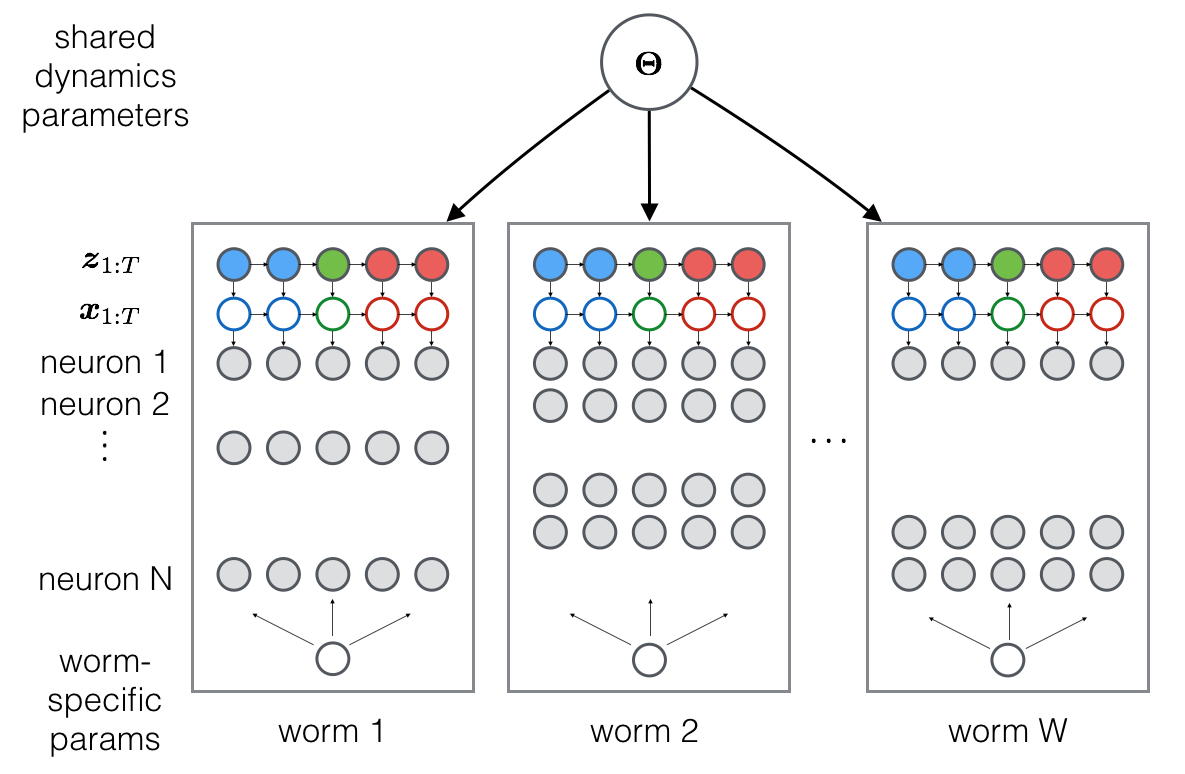
\includegraphics[width=\textwidth]{figures/hslds.png} 
\caption{A schematic of the hierarchical SLDS for combining information
  across multiple worms in order to learn a shared dynamical system
  for \celegans.  We have a set of shared set of model parameters,~$\theta$,
  represented by the large node at the top of the graphical model. Each
  worm,~$w$ has its own set of discrete latent states (colored nodes)
  and continuous latent states (nodes with colored outlines) and observed neurons.
  For example, neuron~1 may appear in all neurons whereas neuron~2
  may only be seen in worm~2. Thus, each worm provides information
  about the mapping from latent states to observations for only a
  subset of neurons. In terms of the model, this corresponds to a
  subset of rows in the matrix~$C$ and the vector~$d$. Finally,
  we allow each worm to have local parameters that capture, for example,
  the amount of fluorescent protein expressed in a particular neuron
  for a given worm. 
}
\label{fig:hslds}
\end{figure}

\subsection{Extensions of the standard SLDS}
\label{sec:extensions}

To better model the \celegans~data, we introduce three extensions
to the standard SLDS.

\paragraph{Hierarchical model to allow limited variability across worms.}
The first extension captures shared patterns across worms while
still allowing for worm-to-worm variability.  We do this in
two ways. First, we allow the dynamics parameters to vary
slightly from worm to worm with the following model,
\begin{align*}
  \mathrm{vec}([A_k, b_k]) &\sim \distNormal(\lambda), \\
  \mathrm{vec}([A_k^{(w)}, b_k^{(w)}]) &\sim \distNormal(\mathrm{vec}([A_k, b_k]), \sigma^2 I), \\
  Q_k^{(w)} &\sim \mathrm{IW}(\lambda).
\end{align*}
This allows worm-specific dynamics parameters~$(A_k^{(w)}, b_k^{(w)})$ but
requires that they not deviate too far from the global mean~$(A_k, b_k)$.
It also allows for worm-specific dynamics noise. 

Second, we allow each worm to have neuron-specific emission variances,
\begin{align*}
  s_{n}^{(w)} & \iid\sim \mathrm{IG}(\eta).
\end{align*}
We may expect, for example, that calcium indicator expression
varies from worm to worm, which in turn could give rise to
different levels of observed activity.  While this could be
modeled as a scaling of the emission matrix, a simpler approach
is to let the noise term capture these different fluctuations.
We could share the global mean of the worm-specific variances,
but we have little reason to expect the~$s_{n}^{(w)}$ and~$s_{n}^{(w')}$
to be correlated under the prior. 

Figure~\ref{fig:hslds} illustrates the hierarchical model.  Each
worm has a set of discrete states~$z_{1:T}$, continuous states~$x_{1:T}$,
and observations for a subset of neurons.  The worms share a set of
global dynamics parameters and emission matrices, but they also
have worm-specific perturbations of the global dynamics, as well as
worm-specific observation variances. 

\paragraph{Robust dynamics model.}  While the SLDS can capture nonlinear
dynamics by composing simple linear pieces, it is still an approximation
to the true data-generating process.  To account for some of this
model misspecification, we introduce a \emph{robust} extension of the
SLDS by allowing for heavy-tailed noise in the dynamics.  Specifically,
we replace~\eqref{eq:slds_start} with,
\begin{align}
  x_{t+1}^{(w)} &= A_{z_{t+1}^{(w)}} x_{t}^{(w)} + b_{z_{t+1}^{(w)}} +  u_t^{(w)},
  &
  u_t^{(w)} &\iid\sim \mathrm{t}(0, Q_{z_{t+1}^{(w)}}, \nu_{z_{t+1}^{(w)}}),
\end{align}
where~$\mathrm{t}(\cdot, \cdot, \cdot)$ denotes the multivariate-t
distribution.  This distribution has heavier tails than its Gaussian
counterpart; indeed, it can be derived by a mixture of multivariate
Gaussians with a~$\chi^2$-distributed scaling of the covariance matrix. 

\paragraph{Recurrent model of discrete state transition probabilities.}
Finally, we consider a third extension that allows for more complex
transition probabilities.  We replace~\eqref{eq:markov_z} with,
\begin{align}
  z_{t+1}^{(w)} \given z_t^{(w)}, x_t^{(w)}
  &\sim \mathrm{softmax}(r_{z_t^{(w)}} + R x_t^{(w)}),
    \label{eq:recurrent}
\end{align}
where~${r_k \in \reals^K}$ and~${R \in \reals^{K \times D}}$
parameterize a map from previous discrete and continuous states to a
distribution over next discrete states.  The link function is the
softmax function, which exponentiates and normalizes
the~$K$-dimensional argument~${r_{z_t^{(w)}} + R x_t^{(w)}}$.

\section{Model Fitting}

We have proposed a variety of Bayesian algorithms for learning the
model parameters~$\theta$ and performing joint inference of the
latent states~$z$ and~$x$~\citep{linderman2017recurrent, linderman2017structure},
but for simplicity, here we treat inference of~$x$ and~$z$ separately.
That is, first we find low-dimensional continuous states to model the
observations~$y$, then we find a set of discrete states~$z$ that best
explain the dynamics in~$x$. We learn the corresponding parameters
at both stages.


\todo[inline, size=\normalsize]{We will present full details of these inference
procedures in the appendix, but for now, here are a few highlights.}

To be more specific, first we fit linear dynamical systems to infer
the continuous latent states~$x$ given the observed values of~$y$.
Since many entries of~$y$ are masked off, this requires inference
with missing data.  Under the assumption of diagonal observation
covariance, this inference is straightforward.  We will compare the
standard LDS with the hierarchical LDS, which has worm- and neuron-specific
variances.

Once we have inferred the continuous latent states, we will fit
an autoregressive hidden Markov model (AR-HMM) to~$x$ in order
to infer~$z$ and learn the dynamics parameters~$(A_k, b_k, Q_k)$.
Here, again, we will consider all possible variants of hierarchical,
robust, and recurrent models.

Both fitting procedures use Markov chain Monte Carlo, specifically
block Gibbs sampling, to sample from the conditional distribution
of latent states given parameters and of parameters given latent
states.  We run these algorithms for 1000 iterations, at which
point we find them to have converged on the basis of held-out
log likelihood. 



\section{Results}
\label{sec:results}

\todo[inline, size=\normalsize]{For this draft, I will present results one at a time,
  each on a separate page.  Once we have settled on the story, we
  can add more exposition.}
\clearpage

\subsection{Neural activity is low-dimensional and has worm-specific variance}


\begin{figure}[h]
  \centering
  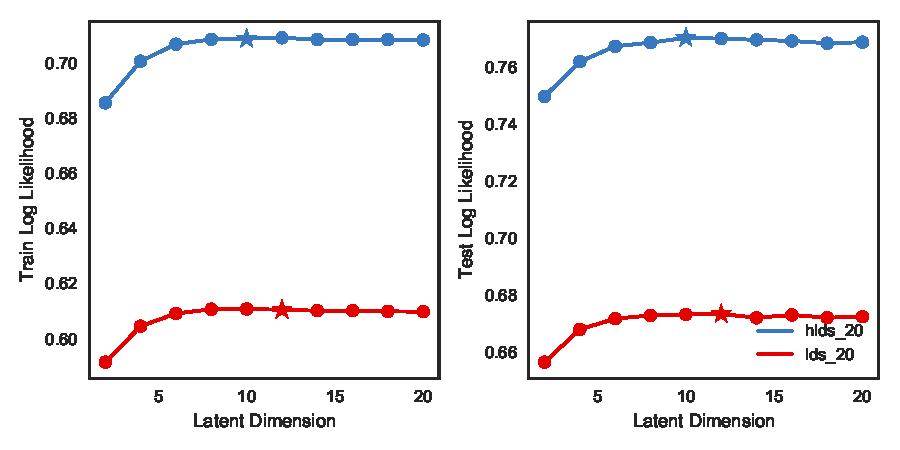
\includegraphics[width=6in]{figures/lds/dimensionality} \\
  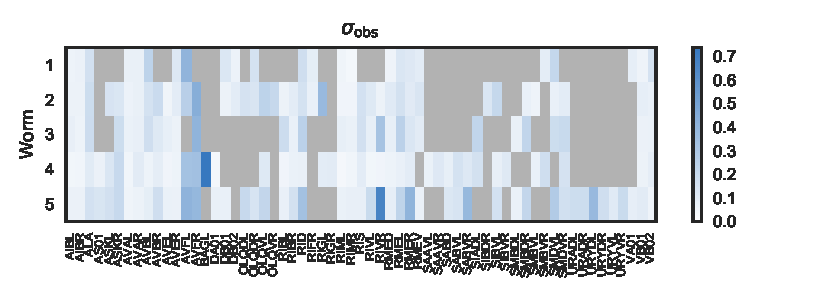
\includegraphics[width=5.5in]{figures/lds/observation_variance} 
  \caption{\textit{(top)} Training and test likelihoods for the linear
    dynamical system and its hierarchical extension as a function of
    the dimensionality of the latent state,~$D$ (units:
    nats/observation over Gaussian baseline). On the basis of held-out
    test likelihood, we choose the hierarchical LDS with
    10-dimensional latent states.  \textit{(bottom)} Inferred standard
    deviation~$\sqrt{s_n^{(w)}}$ for each neuron and worm.  Gray cells
    indicate neurons that were not observed in that worm.}
  \label{fig:lds}
\end{figure}

We fit linear dynamical systems (LDS) and their hierarchical
extensions with worm-specific variance (see Section~\ref{sec:extensions})
for a range of latent dimensions,~$D$.  We found that the
10-dimensional hierarchical LDS yielded the highest test
likelihood (holding out the final 20\% of time frames for
each worm for testing, assuming stationarity). This is
shown in Figure~\ref{fig:lds}(top).

The hierarchical model has worm-specific observation variances.
These are shown in Figure~\ref{fig:lds}(bottom).  For neurons that
were not observed in a given worm, the corresponding cells are
colored gray. 

\clearpage

\subsection{The hierarchical LDS smooths the data and predicts unobserved activity}


\begin{figure}[h]
  \centering
  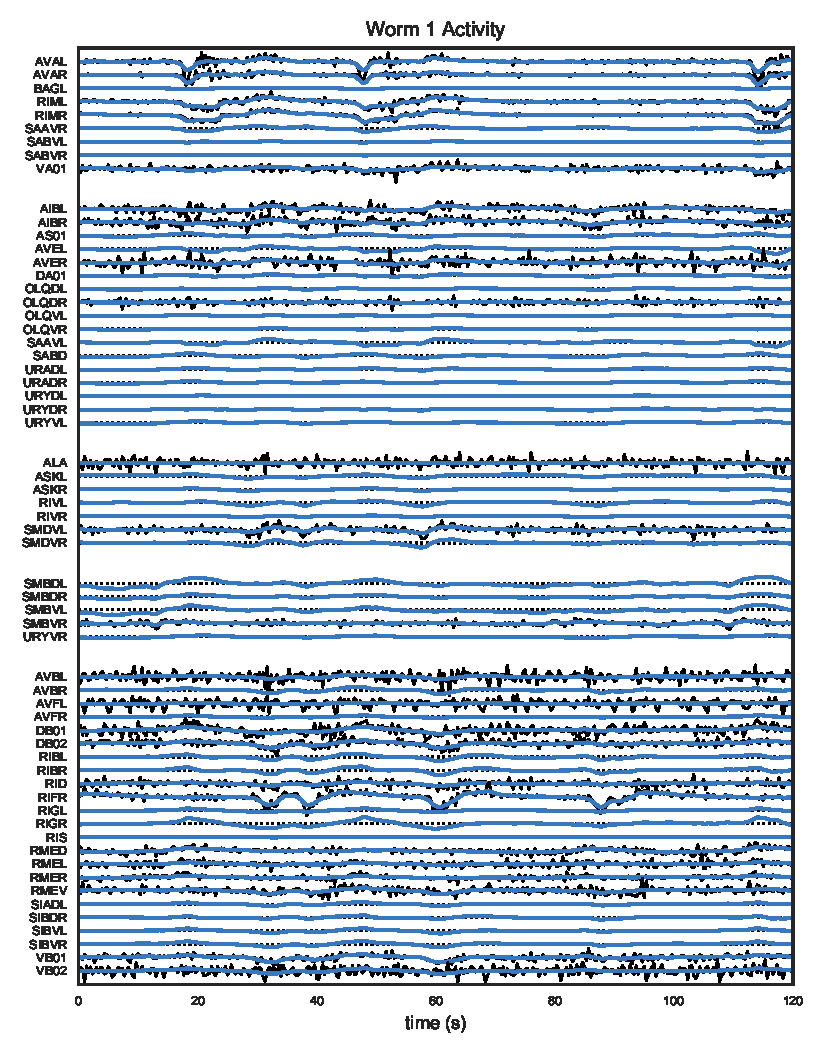
\includegraphics[width=5.5in]{figures/lds/y_0}
  \caption{The observed activity~$y$ (i.e. the first-order differences
    of the calcium signal) are shown in black; the smoothed activity
    with the hierarchical LDS is shown in blue.  The hierarchical LDS
    makes predictions about unobserved neurons---those with dotted
    black lines---based on the correlations found in other worms. We
    show two minutes of data here.  The neurons have been grouped into
    five clusters, as discussed below.  Within each cluster, the
    neurons are sorted alphabetically. Each neuron is individually
    scaled by the standard deviation of its observed activity to
    illustrate dynamics of low-amplitude neurons. }
  \label{fig:activity_1}
\end{figure}

Figures~\ref{fig:activity_1}-\ref{fig:activity_5} show the observed
activity~$y$ along with the smoothed activity under the hierarchical
LDS.  Formally, the blue lines are given by~$C \E[x \given y] +
d$. Unobserved neurons are shown as dotted black lines.  Though their
activity is not observed, the hierarchical model can predict it based
on correlations observed in other worms. 

\begin{figure}[h]
  \centering
  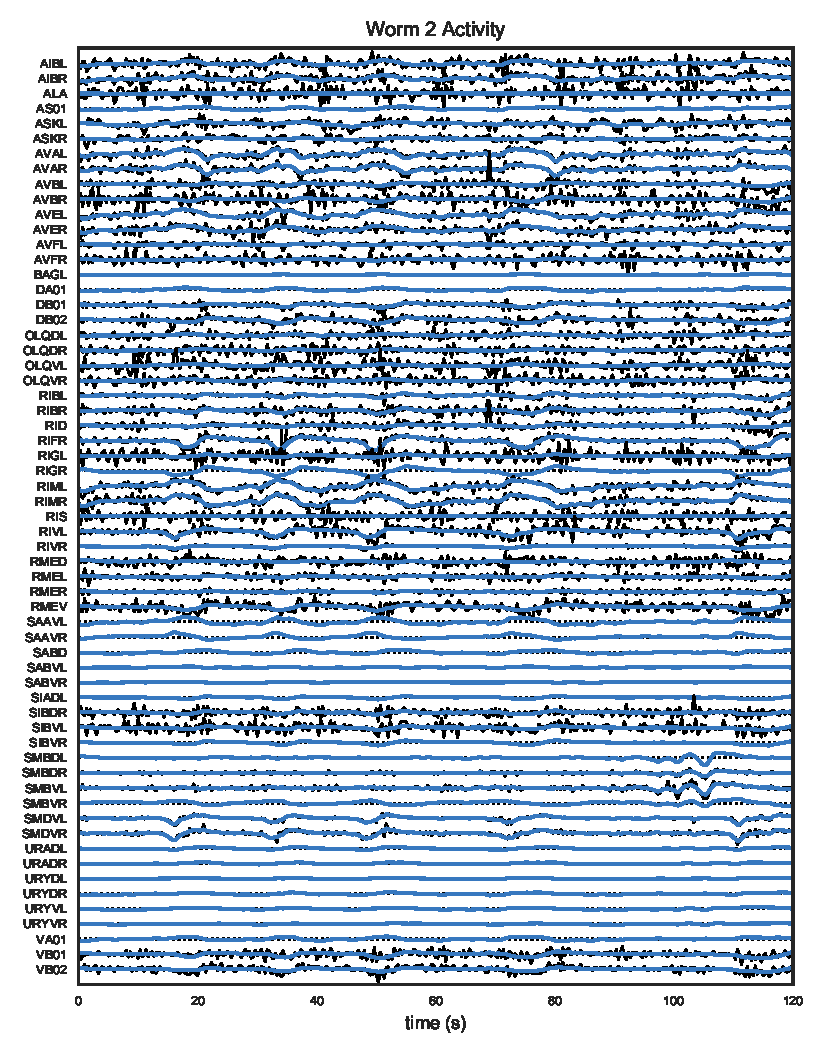
\includegraphics[width=5.5in]{figures/lds/y_1}
  \caption{See caption of Figure~\ref{fig:activity_1}}
  \label{fig:activity_2}
\end{figure}

\begin{figure}[h]
  \centering
  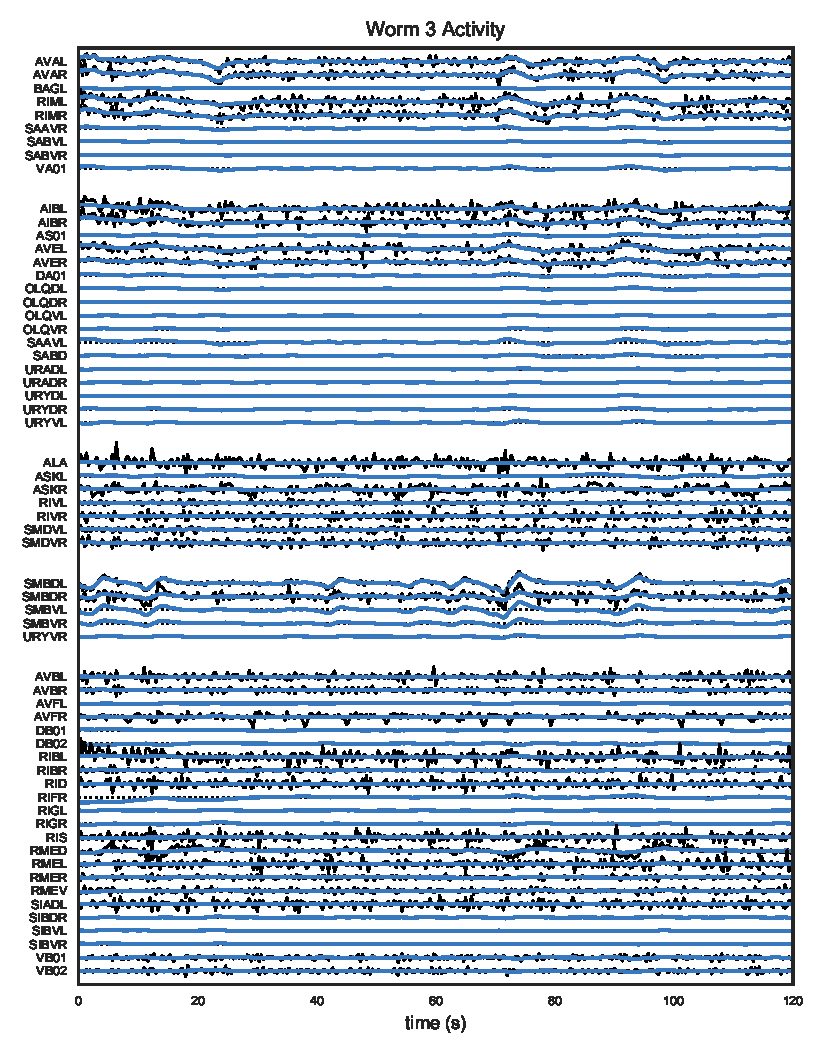
\includegraphics[width=5.5in]{figures/lds/y_2}
  \caption{See caption of Figure~\ref{fig:activity_1}}
  \label{fig:activity_3}
\end{figure}

\begin{figure}[h]
  \centering
  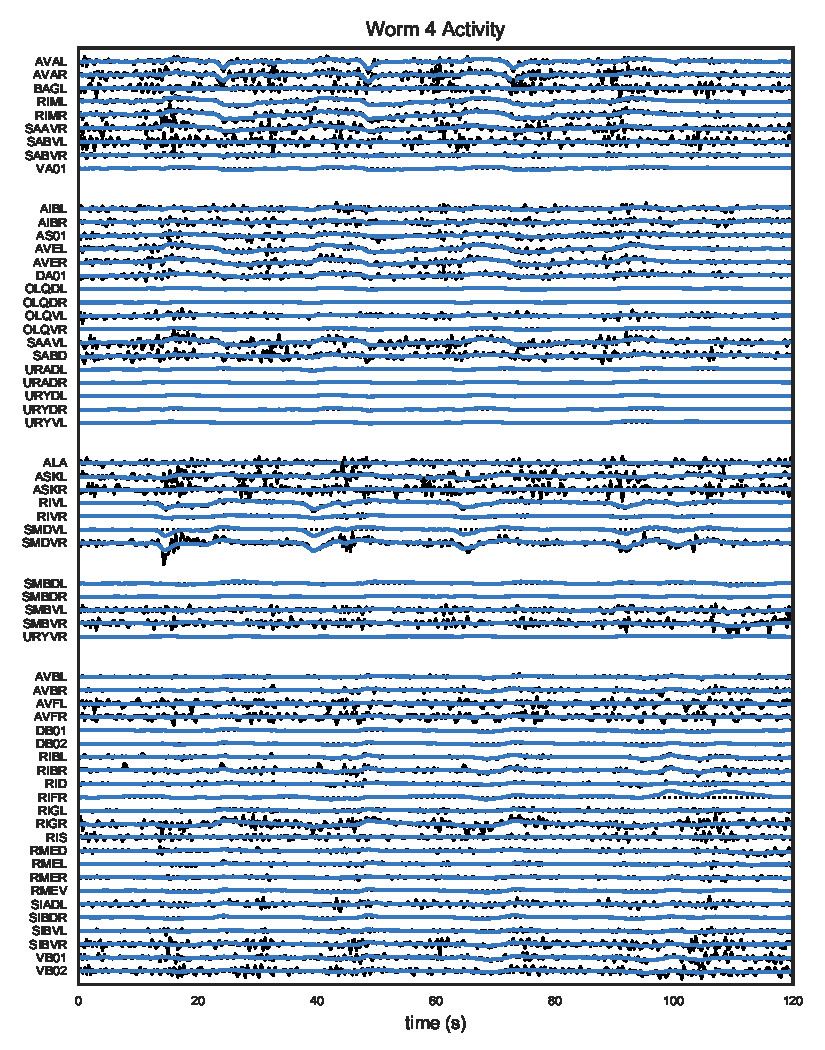
\includegraphics[width=5.5in]{figures/lds/y_3}
  \caption{See caption of Figure~\ref{fig:activity_1}}
  \label{fig:activity_4}
\end{figure}

\begin{figure}[h]
  \centering
  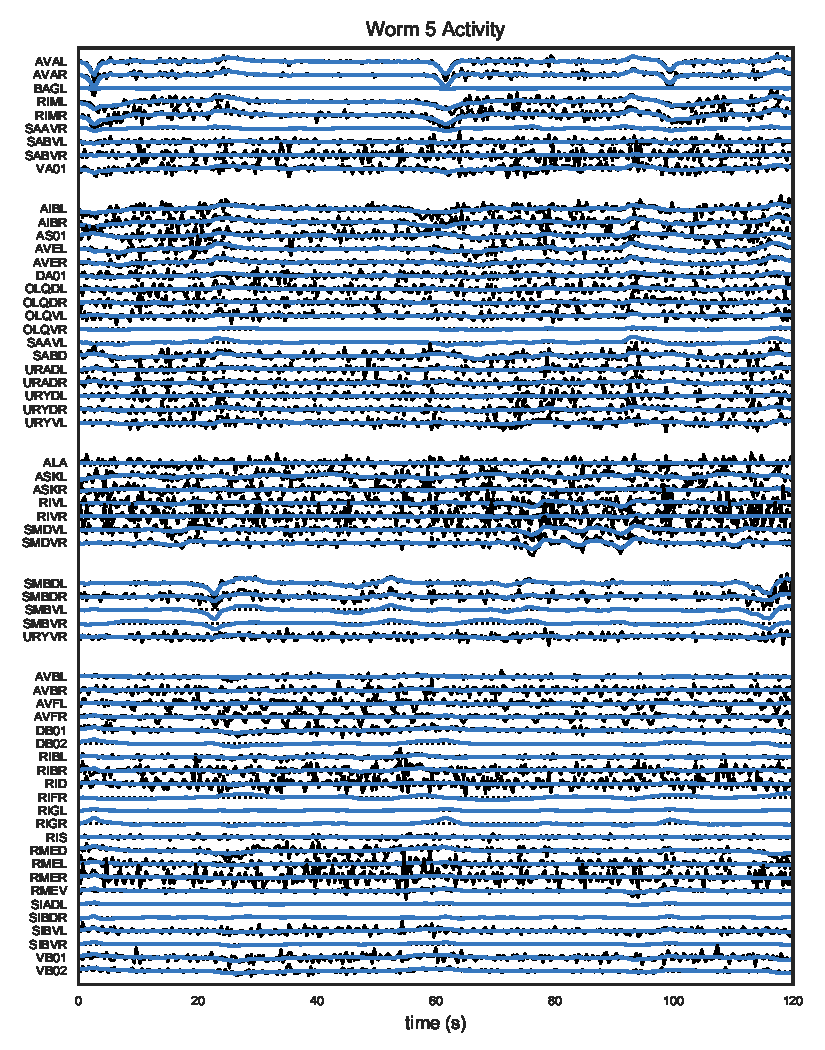
\includegraphics[width=5.5in]{figures/lds/y_4}
  \caption{See caption of Figure~\ref{fig:activity_1}}
  \label{fig:activity_5}
\end{figure}

\clearpage

\subsection{The emission parameters aid in neural identification}

One of the challenges in modeling this data is that most neurons
cannot be labeled with certainty.  In other words, we can detect a
neuron in the calcium imaging data, but we cannot determine its
identity (\textsf{AVAL}, \textsf{AVAR}, etc.).  The emission
parameters of the SLDS are a useful aid for determining these
identities, as we show here.

Across the dataset of five worms, 61 unique neurons were identified in
at least one worm.  In any given worm, we also observe many other
neurons that we cannot accurately label. Our goal here is to assign
labels to the unlabeled neurons.  Of course, if a label, say \textsf{AVAL}, has
already been identified in worm 1, then we cannot assign an unlabeled
neuron to \textsf{AVAL}.  So the problem is to find the most likely matching
of unlabeled neurons to remaining, available labels.  Since there are
more unlabeled neurons than possible labels, our result will only be
a partial matching. 

The rows of the emission matrix~$c_n$ serve as ``embeddings'' of the
neurons. These embeddings can aid in this matching.  Specifically,
given an activity trace~$y^{(w)}_{n^*} \in \reals^T$ for an unlabeled
neuron~$n^*$ in worm~$w$, along with the set of continuous latent
states~$x^{(w)} \in \reals^{T \times D}$ inferred from the labeled
neurons, we perform a linear regression to
estimate~$c_{n^*} \in \reals^D$, the ``embedding'' of this unlabeled
neuron.  We then compare this vector~$c_{n^*}$ to the embeddings of
the labeled neurons,~$\{c_n\}_{n=1}^N$, which were learned with the
SLDS.  We use the cosine similarity between two vectors as a measure
of likeness.


\begin{figure}[h]
\centering%
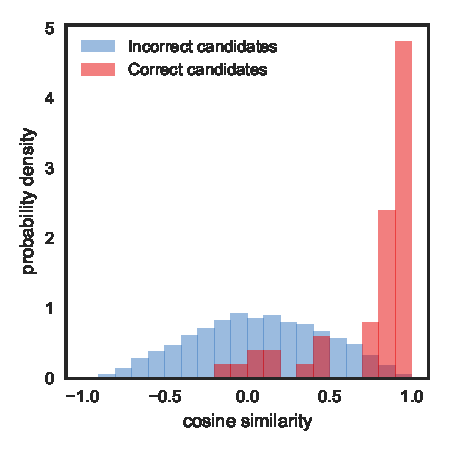
\includegraphics[width=3in]{figures/lds/similarity_comparison} 
\caption{The emission parameters aid in neural identification.  In
  this task, we view unlabeled neurons as \emph{candidates} for a
  particular label. For example, suppose we are trying to determine
  the candidate neuron that is most likely to be~\textsf{AVAL}. For
  this task, we have artificially held-out this label so that we know
  which candidates truly is~\textsf{AVAL}. We use the neural
  embeddings~$c_{\mathsf{AVAL}}$, which was inferred from other worms,
  to aid in this matching.  We measure the cosine similarity
  between~$c_{\mathsf{AVAL}}$ and the coefficients of linear
  regressions between~$x$ and the activity of the unlabeled neurons'
  activity. This histogram shows the results of performing this
  experiment with 10 held-out identities for each of the five worms.
  We see that the correct candidates frequently have much higher
  cosine similarity than incorrect candidates.  This means that we can
  use this similarity measure to infer neuron identities.  }
\label{fig:neuron_id}
\end{figure}

We demonstrate this identification in a synthetic task where we
artificially withheld the labels of ten neurons per worm.  Suppose one
of the held-out neurons in worm 1 was known to be \textsf{AVAL}.  We
iterate through all the unlabeled neurons in worm
1---\emph{candidates} for the label~\textsf{AVAL}---and measure the
cosine similarity between their embeddings~$c_{n^*}$ and the
embedding~$c_{\mathsf{AVAL}}$, which was inferred from worms 2-5.
Figure~\ref{fig:neuron_id} shows the results of this task.  The
embeddings of the held-out neurons were much more similar to the
embedding of their true identity than were the other unlabeled
neurons.


To further quantify these results, we sort these similarities
and find the index of the true held-out neuron in the sorted list.
If the held-out AVAL neuron was the most similar to~$c_{\mathsf{AVAL}}$,
its rank would be 1; if it was the least similar, its rank would
be~$N_{\mathsf{unlabeled}}$, the number of unlabeled neurons for
this worm.  Table~\ref{tab:neuron_id} shows the ranks of the
similarities of held-out neurons to their true identities, compared
to all other unlabeled neurons.  If the held-out
neurons were always the most similar to their true embeddings, the
matching columns would all be 1's, and we would easily be able to
identify neurons with this information.  We see that in most cases
the held-out neurons are within the top three most similar candidates,
demonstrating that embeddings are useful for identification. 


Finally, we perform an even harder task. Using the Hungarian algorithm,
we find the partial matching that maximizes the sum of similarities.
We compute the accuracy of this matching by counting the fraction of held-out
neurons that were assigned to their true label. (Since the Hungarian
algorithm is assigning all the neurons at once, in general the number
of correctly assigned neurons is not equal to the sum of 1's in the
rank columns.) Still, we see that in this challenging task we assign
many neurons to their true identities.


\begin{table}[h]
  \caption{\textit{Artificial neuron identification task results.}  In
    each worm we have~$N_{\mathsf{labeled}}$ labeled neurons
    and~$N_{\mathsf{unlabeled}}$ unlabeled neurons. Of the unlabeled
    neurons, 10 had known labels that were held out for this task.  We
    compare the cosine similarity of the unlabeled neuron embeddings
    to the embeddings of the labeled neurons, sort the similarities,
    and compute the rank of each held-out neuron to its true label
    (most similar~=~1; least similar~=~$N_{\mathsf{unlabeled}}$).  We
    use the Hungarian algorithm to find the most likely matching of
    unlabeled neurons to possible labels, and we report the fraction
    of the 10 held-out neurons that were correctly matched~(``Acc.'').
  }
  \vspace{1em}
  \label{tab:neuron_id}
  \centering
  \begin{tabular}{cccccccccccccc}
    \toprule
    & $N_{\mathsf{labeled}}$ & $N_{\mathsf{unlabeled}}$ & \multicolumn{10}{c}{Matching Rank (10 Held-out Neurons)} & Acc. \\
    \cmidrule(r){2-2}
    \cmidrule(rl){3-3}
    \cmidrule(rl){4-13}
    \cmidrule(l){14-14}
    % \midrule
    Worm 1 & 14 & 95 & 10 & 25 & 1 & 1 & 66 & 2 & 1 & 1 & 2 & 1 & 0.30 \\
    Worm 2 & 31 & 76 & 3 & 1 & 1 & 1 & 1 & 39 & 1 & 1 & 1 & 4 & 0.50 \\
    Worm 3 & 20 & 111 & 5 & 53 & 3 & 22 & 1 & 2 & 1 & 1 & 1 & 1 & 0.50 \\
    Worm 4 &33 & 93 & 2 & 1 & 26 & 2 & 1 & 56 & 1 & 1 & 1 & 1 & 0.30 \\
    Worm 5 & 38 & 91 & 1 & 1 & 1 & 1 & 1 & 2 & 1 & 26 & 1 & 67 & 0.70 \\
    \bottomrule
  \end{tabular}
\end{table}

\clearpage

\subsection{Neural embeddings reveal clusters of similarly tuned neurons}

\begin{figure}[h]
\centering%
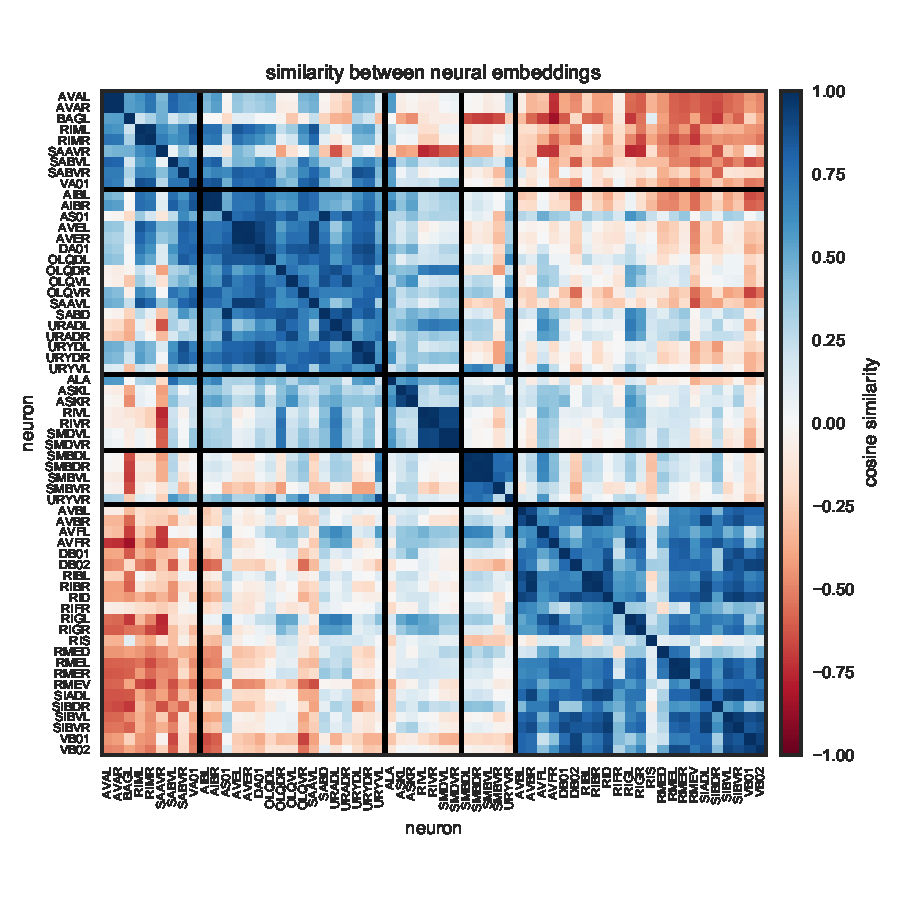
\includegraphics[width=5.5in]{figures/lds/permuted_similarity}
\vspace{-3em}
\caption{Cosine similarity between embedding vectors~$c_n$
  suggest clusters of similarly tuned neurons. }
\label{fig:clusters}
\end{figure}

The rows of the emission matrix~$c_n$ (i.e. the embedding vectors)
also suggest that neurons cluster into groups of similarly tuned
cells.  Figure~\ref{fig:clusters} shows the~${N \times N}$ matrix of
cosine similarity for each pair of embedding vectors.  We used k-means
to find clusters of embedding vectors and have permuted the
similarity matrix to visualize these groups.  We see that many
clusters contain lateral pairs (e.g. {\sf AVAL, AVAR} in
the first cluster). 
We will use these clusters to better understand the dynamics of
the SLDS.

Note that this clustering is not so simple without a hierarchical model.
Since we never see all 61 neurons in a single worm, we need some means
of combining information across worms in order to cluster their activity.
The hierarchical LDS does exactly this.  We could consider simpler
hierarchical models, e.g. a hierarchical factor analysis model that does
not include assumptions about temporal dynamics; such a model would
probably yield similar clusters.  The key point is that we must combine
information across worms.

\clearpage

\subsection{Latent dynamics are hierarchical, robust, and recurrent}

\begin{figure}[h]
\centering%
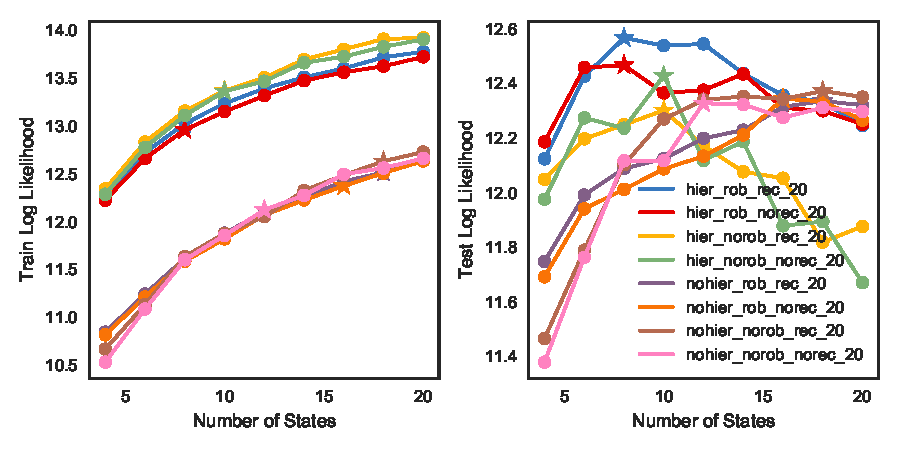
\includegraphics[width=\textwidth]{figures/arhmm/dimensionality.pdf} 
\caption{Training and test likelihood of the hierarchical
  autoregressive hidden Markov models (a special case of the SLDS) for
  all combinations of hierarchical, robust, and recurrent extensions.
  We evaluate test likelihoods for a range of numbers of latent
  states, and we find that the hierarchical, robust, recurrent model
  with~$K=8$ latent states performs best.}
\label{fig:arhmm_lls}
\end{figure}

As with the LDS, we fit autoregressive hidden Markov models (AR-HMMs)
with all combinations of hierarchical, robust, and recurrent extensions
described in Section~\ref{sec:extensions}.  For each possible model, we
swept from~$K=2$ to~$K=20$ discrete latent states in increments of two.

Overall, the hierarchical models (red, blue, yellow, green) performed
best across all~$K$ in training data.  This is not surprising as the
hierarchical models effectively have~$W \cdot K$ dynamics
parameters---one version of each state for each worm---whereas the
non-hierarchical models have only~$K$.  Of these hierarchical models,
only those with the robust extension showed good generalization.  The
non-robust models (with standard Gaussian noise; green, yellow)
severely overfit the training data.  Of the robust hierarchical models,
the recurrent model showed substantial improvement over the non-recurrent
model, and obtained peak performance with~$K=8$ states.  Likelihoods
are measured in units of nats/time step.

\clearpage

\subsection{The AR-HMM automatically segments low-dimensional states}

\begin{figure}[h]
\centering%
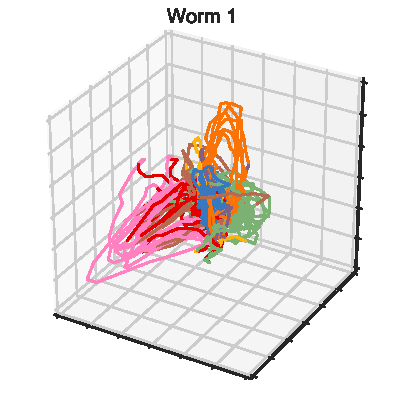
\includegraphics[width=2.7in]{figures/arhmm/x_3d_1.pdf}
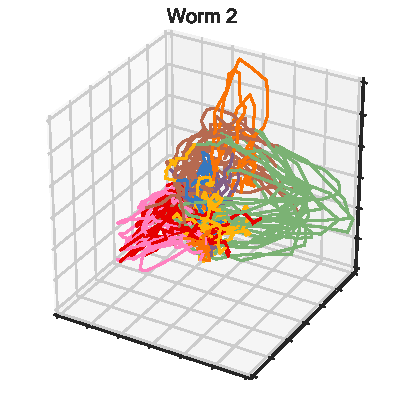
\includegraphics[width=2.7in]{figures/arhmm/x_3d_2.pdf}
\\
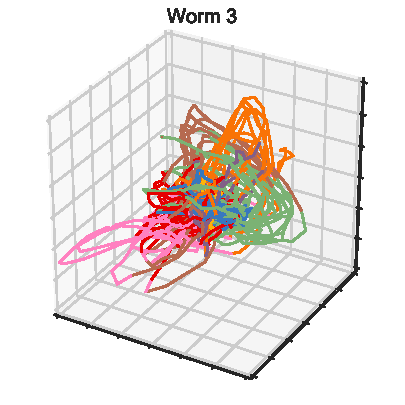
\includegraphics[width=2.7in]{figures/arhmm/x_3d_3.pdf}
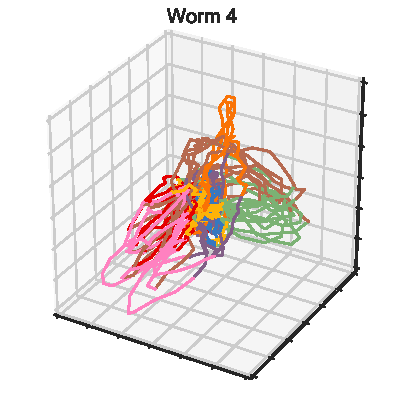
\includegraphics[width=2.7in]{figures/arhmm/x_3d_4.pdf}
\\
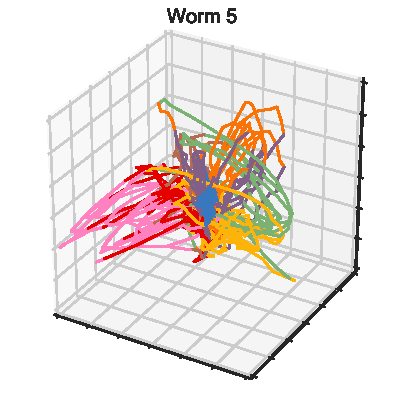
\includegraphics[width=2.7in]{figures/arhmm/x_3d_5.pdf} 
\caption{Three dimensional projections of the 10 dimensional
  latent states~$x$. The trajectories are color coded
  according to the inferred discrete states~$z$.  We find
  that discrete states correspond to different ``loops''
  in latent space, and that they are, to large extent,
  used in separate regions of~$x$-space.  This is consistent
  with the recurrent model.}
\end{figure}

Since the continuous latent states are 10 dimensional, we use only the
three dimensions of activity for visualization.  We choose the three
dimensions that are most correlated with the observed neural activity.
We color code these three-dimensional trajectories according to the
discrete states~$z$, which correspond to different linear dynamical
regimes of the continuous states~$x$. Compare these plots to the state
space plots of~\citet{kato2015global}. These trajectories are not as
smooth (which is expected given that we are modeling the first-order
differences directly), but they capture the same qualitative patterns.
We will quantify this correspondence shortly. 

\clearpage

\subsection{The AR-HMM learns dynamical systems for each discrete state}

\begin{figure}[h]
\centering%
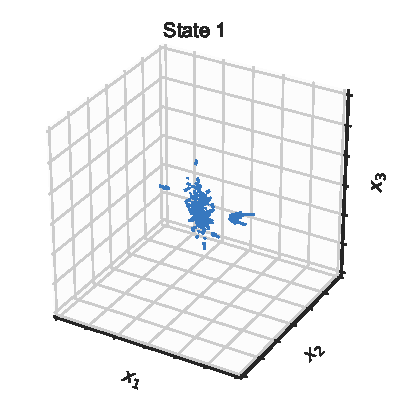
\includegraphics[width=2.7in]{figures/arhmm/dynamics_123_0.pdf}
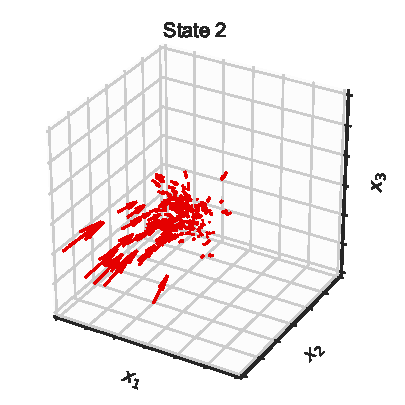
\includegraphics[width=2.7in]{figures/arhmm/dynamics_123_1.pdf}
\\
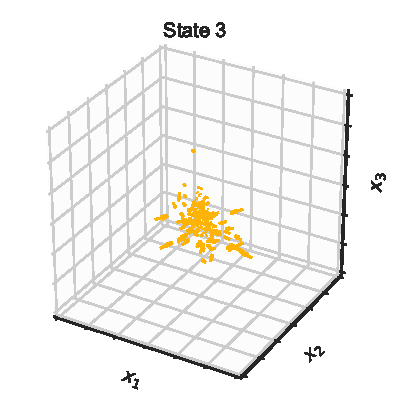
\includegraphics[width=2.7in]{figures/arhmm/dynamics_123_2.pdf}
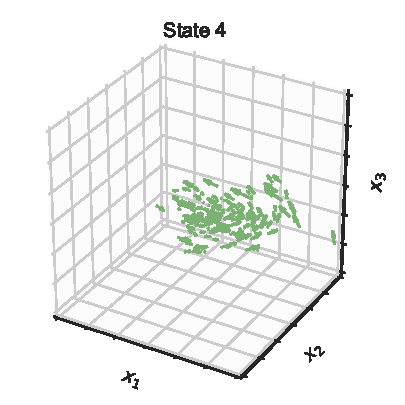
\includegraphics[width=2.7in]{figures/arhmm/dynamics_123_3.pdf}
\caption{Each discrete state has a corresponding set of linear dynamics
  parameters~$(A_k, b_k)$, which we visualize here as a vector field.
  Each arrow shows where a point~$x_t$ would be mapped to by the 
  linear dynamics of a given state. We visualize points~$x_t$ where
  the states were actually used. We see a number of states related
  to ``returning to the origin'' (e.g. states 1, 2, 3, 5), as well
  as states corresponding to loops (e.g. states 4, 6, 7).}
\label{fig:dynamics}
\end{figure}

\begin{figure}[h]
  \centering%
  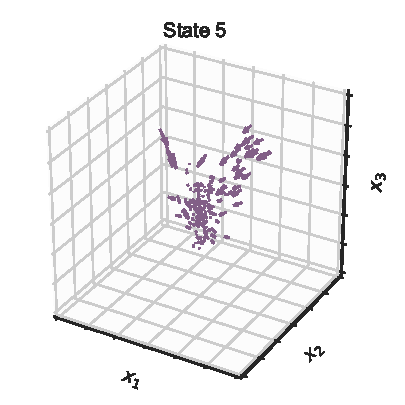
\includegraphics[width=2.7in]{figures/arhmm/dynamics_123_4.pdf}
  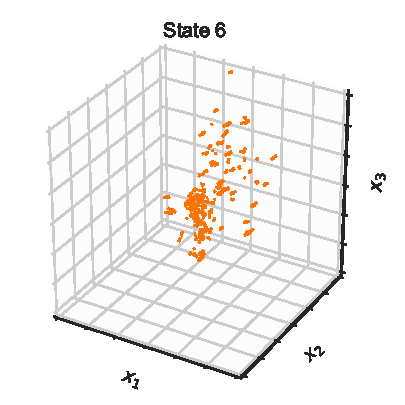
\includegraphics[width=2.7in]{figures/arhmm/dynamics_123_5.pdf}
  \\
  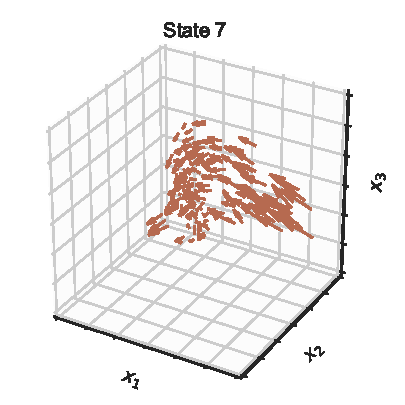
\includegraphics[width=2.7in]{figures/arhmm/dynamics_123_6.pdf}
  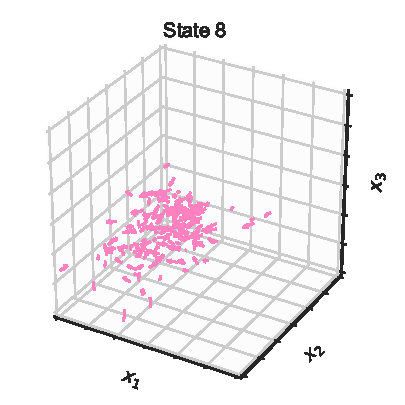
\includegraphics[width=2.7in]{figures/arhmm/dynamics_123_7.pdf}
  \caption{See caption for Figure~\ref{fig:dynamics}}
  \label{fig:dynamics2}
\end{figure}
Figures~\ref{fig:dynamics} and~\ref{fig:dynamics2} illustrate the
global dynamics parameters for each of the~$K$ discrete states.
Specifically, we show where a point~$x_t$ would be mapped to by the
operation~$A_k x_t + b_k$.  We choose a subset of starting
points~$x_t$ where the discrete state was used. Many of the states
correspond to returning to the origin, which in turn corresponds to
constant neural activity (since we are modeling the first-order
differences in the calcium signal).  Other states correspond to loops,
which give rise to increases in the activity of some clusters of
neurons and decreases in others.

\clearpage

\subsection{Inferred states correspond to activation of clusters of neurons}


\begin{figure}[h]
\centering%
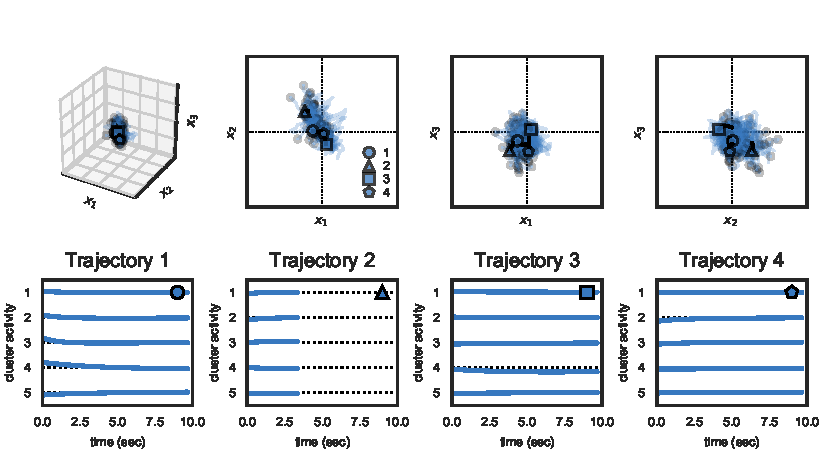
\includegraphics[width=5in]{figures/arhmm/cluster_activity_0.pdf}
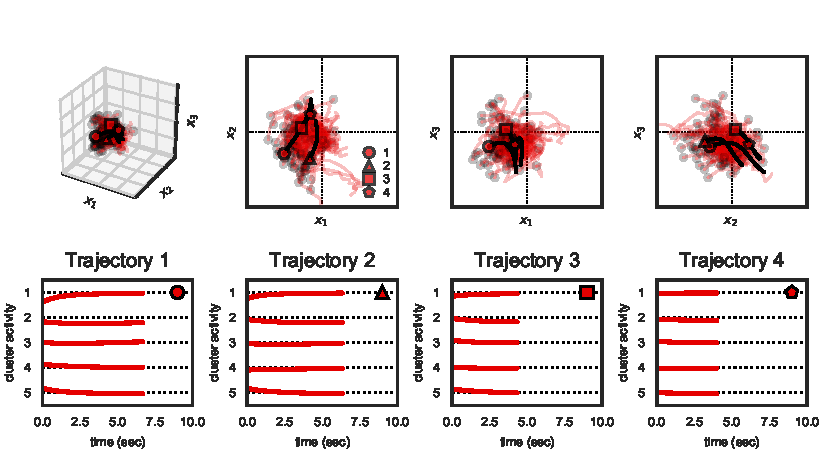
\includegraphics[width=5in]{figures/arhmm/cluster_activity_1.pdf}
\caption{(top) Colored traces show a number of real-data trajectories
  that were inferred to be in states 1 (blue) and 2 (red).  Then we
  simulate from our model's inferred linear dynamical system for these
  states, and show simulated trajectories with four different starting
  points (circle, triangle, square, and pentagon) in black lines.
  The top left panel shows the top 3 dimensions of these trajectories
  in latent state space. The
  top right panels show 2D views of the same trajectories.  (bottom)
  These four simulated trajectories give rise to different patterns of
  neural activity in the five inferred clusters.  For example, the
  first trajectory of the second state (red circle) corresponds to
  activity that decays toward the baseline for each of the clusters,
  with a starting value of below-baseline activity in the first
  cluster.}
\label{fig:cluster_activity_12}
\end{figure}

Figures~\ref{fig:cluster_activity_12}, \ref{fig:cluster_activity_34},
\ref{fig:cluster_activity_56}, and~\ref{fig:cluster_activity_78} show
how trajectories in continuous latent state space for each of the~$K$
states manifest in the activity of the neural clusters identified in
Figure~\ref{fig:clusters}.  The black lines with circle, triangle,
square, and pentagon starting points are forward simulated
trajectories using the inferred dynamics of state~$k$ with four
different initial conditions. The initial conditions are values
of~$x_t$ where we had inferred an entry into state~$k$.
The bottom rows show how the activity the forward
simulated trajectories activate each of the five clusters of
neurons.

The colored lines in the top panel are segments of~$x$ that were
inferred to be in state~$k$.  Recall that these continuous latent
states were found by first fitting a hierarchical LDS. As such, they
correspond to the conditional mean of the posterior
distribution under the hierarchical LDS,~$\E[x \given y]$.

\begin{figure}[h]
\centering%
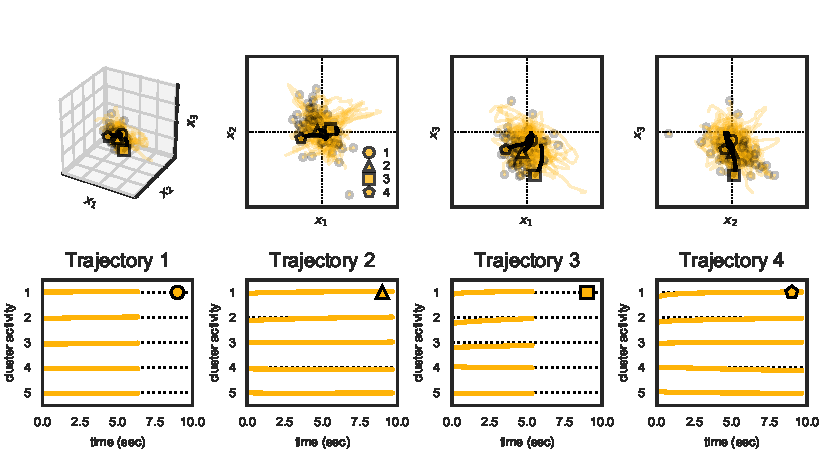
\includegraphics[width=5in]{figures/arhmm/cluster_activity_2.pdf}
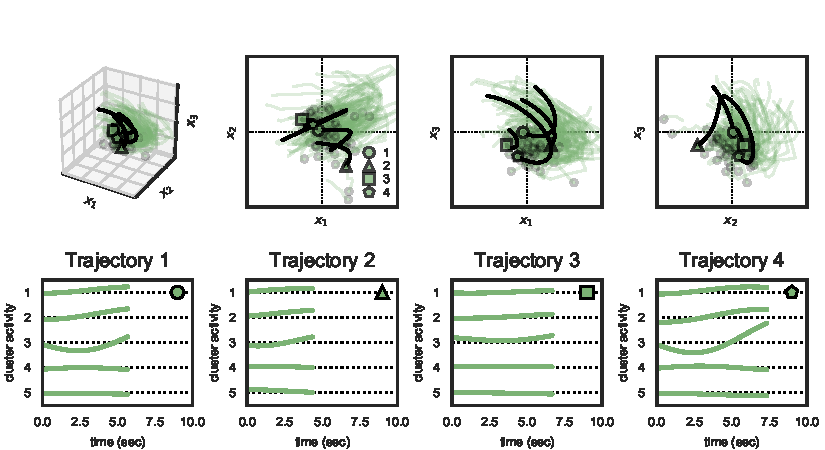
\includegraphics[width=5in]{figures/arhmm/cluster_activity_3.pdf}
\caption{See Figure~\ref{fig:cluster_activity_12} caption.}
\label{fig:cluster_activity_34}
\end{figure}

\begin{figure}[h]
\centering
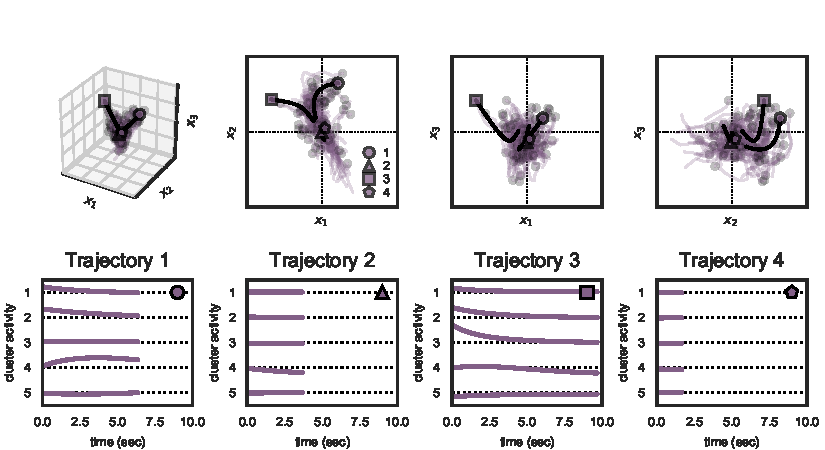
\includegraphics[width=5in]{figures/arhmm/cluster_activity_4.pdf}
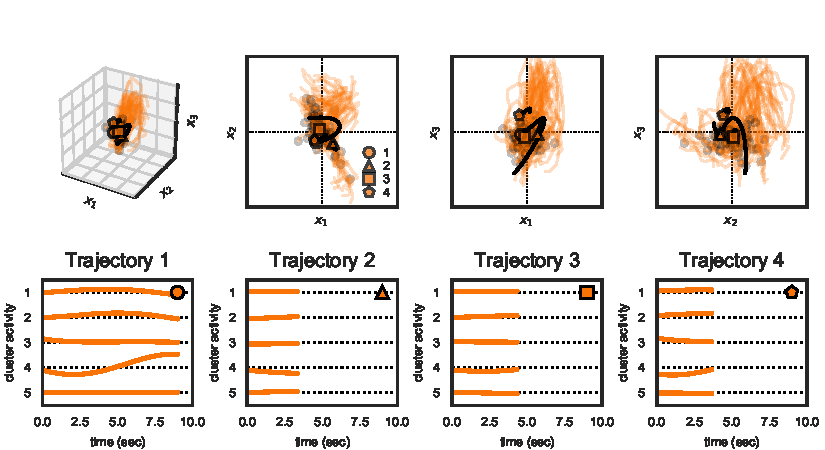
\includegraphics[width=5in]{figures/arhmm/cluster_activity_5.pdf}
\caption{See Figure~\ref{fig:cluster_activity_12} caption.}
\label{fig:cluster_activity_56}
\end{figure}

\begin{figure}[h]
\centering
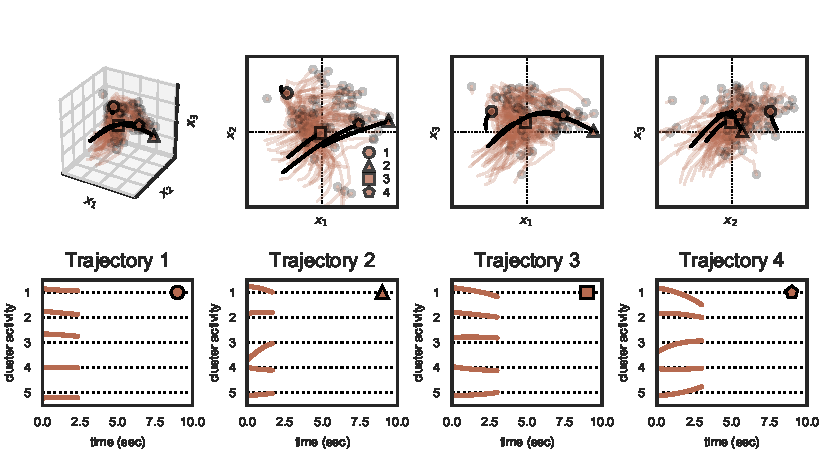
\includegraphics[width=5in]{figures/arhmm/cluster_activity_6.pdf}
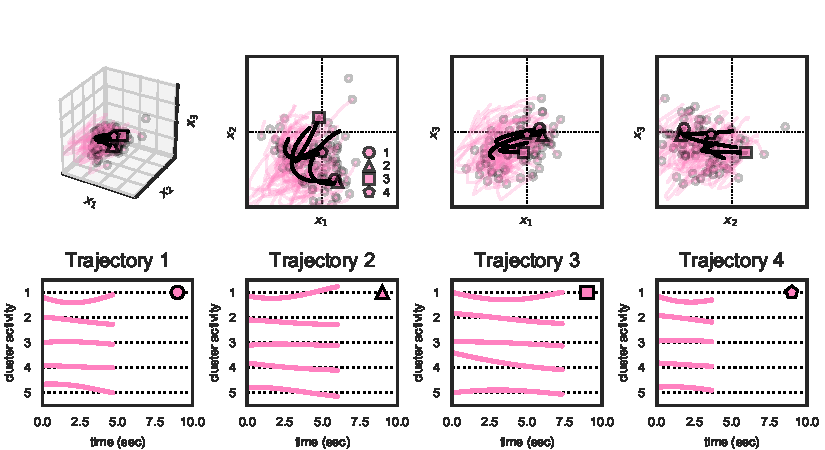
\includegraphics[width=5in]{figures/arhmm/cluster_activity_7.pdf}
\caption{See Figure~\ref{fig:cluster_activity_12} caption.}
\label{fig:cluster_activity_78}
\end{figure}

\clearpage

\subsection{States are employed roughly equally by these worms}

\begin{figure}[h]
\centering
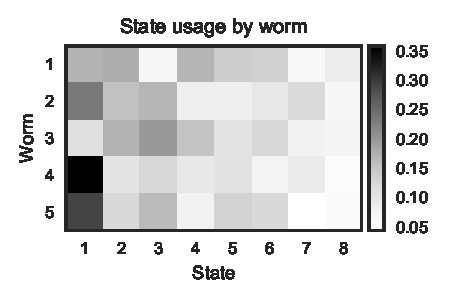
\includegraphics[width=3in]{figures/arhmm/state_usage_per_worm2.pdf}
\caption{Proportion of time frames spent in each state, broken down per-worm.}
\label{fig:usage}
\end{figure}

The worms appear to use these states with roughly equal proportion,
as shown in Figure~\ref{fig:usage}.  The states have been ordered to
overall population usage, but within worms we see that some states
are used slightly more often than others.  For example, worm 3 uses
state 1 less often than the others, and instead seems to have a higher
usage of state 3.  This particular difference is probably not important, but it
points to how these types of methods could be useful for distinguishing
between, for example, different genetic variants of worms.

\clearpage

\subsection{Transition structure is largely stereotyped across worms as well}


\begin{figure}[h]
\centering
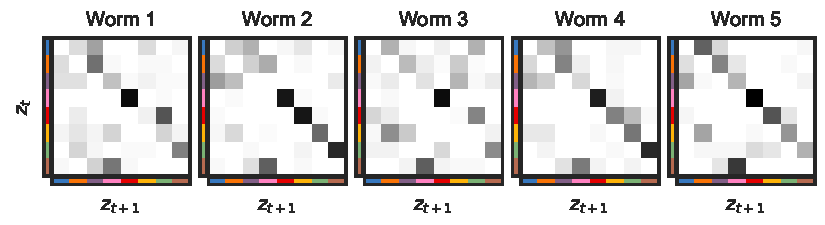
\includegraphics[width=5.5in]{figures/arhmm/trans_matrices.pdf}
\caption{Empirical transition probabilities for each of the worms.  By far
  the most common transition is into the same state.  For visualization, we
  have removed this diagonal component and renormalized so that the~$k$-th row of
  each transition matrix shows the conditional distribution over~$z_{t+1}$ given
  that~$z_{t}=k$ and~$z_{t+1} \neq z_t$. }
\label{fig:trans}
\end{figure}

Figure~\ref{fig:trans} shows the empirical transition matrices for each of the
worms.  We see a few transitions appear across all worms:
\begin{itemize}
\item Pink transitions to red with high probability in all worms. This is evident
  from the state trajectories above.
\item Brown transitions to pink or, with lower probability, to purple.
\item Orange transitions to purple, pink, or blue.
\item Purple and orange transition to blue for most worms, except in worm three,
  which uses yellow in place of blue (see above).
\item Green transitions to brown with high probability across all worms. 
\item For worms 2, 4, and 5, red often transitions into yellow and yellow to green or orange
  for most worms.
\item Blue (the ``origin'' state), tends to transition to purple or orange in
  worms 2, 4, and 5.
\end{itemize}

These aren't meaningful yet, but as we show next, these discrete states closely
match the states identified in~\citep{kato2015global}. 

\clearpage

\subsection{Recurrent weights influence transition probabilities}

\begin{figure}[h]
\centering%
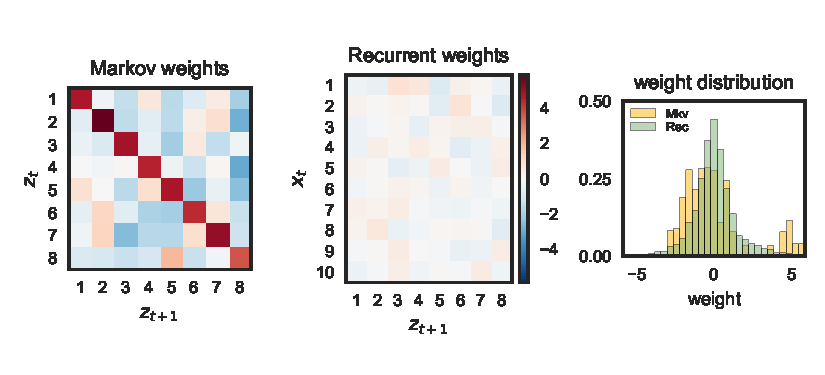
\includegraphics[width=5.5in]{figures/arhmm/recurrent_weights.pdf}
\caption{Weights of the recurrent transition model.  The largest
  weights come from the Markov terms for~$z_{t}$, but the weights
  for the continuous location~$x_t$ are non-trivial.  When we
  compute the effective weights that come from~$r_{z_t}$ and
  the ``recurrent'' terms~$R^\trans x_t$, we see that the recurrent terms
  are a significant fraction of the Markovian terms. }
\label{fig:rec_weights}
\end{figure}

Figure~\ref{fig:rec_weights} shows the two terms that go into the
distribution over next states: the ``Markov'' term~$\{r_{k}\}_{k=1}^K$
and the ``recurrent'' weights~$R$, as defined in
Eq.~\eqref{eq:recurrent}.  Since the impact of the recurrent weights
depends on the scale of the continuous latent states, we multiply the
weight matrix~$R$ by the standard deviation of~$x$ (since~$x$ is
roughly zero mean, this is like z-scoring~$x$ so that it is comparable
with the Markov term).  The largest weights come from the
self-transitions, i.e. the diagonal of the Markov terms. Still, the
recurrent weights are non-negligible. The histogram of Markov
weights~($r_{z_t}$) and the recurrent weights~($R^\trans x_t$) at the
times of transitions (right panel) shows that the recurrent weights
are comparable to the Markov weights, and therefore must play a role
in determining transition probabilities.  This must be the case as the
recurrent models yield significant improvement in held-out log
likelihoods, as shown in Figure~\ref{fig:arhmm_lls}.

\clearpage

\subsection{The recurrent model captures non-Markovian state durations}

\begin{figure}[h]
\centering%
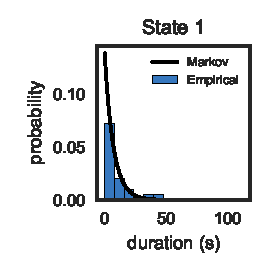
\includegraphics[width=1.8in]{figures/arhmm/durations_0.pdf}
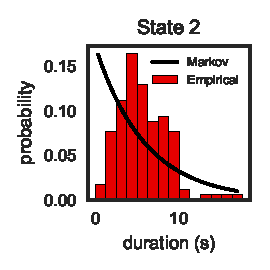
\includegraphics[width=1.8in]{figures/arhmm/durations_1.pdf}
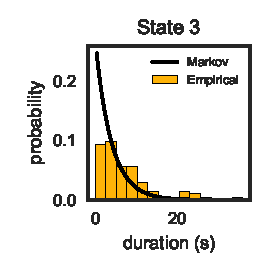
\includegraphics[width=1.8in]{figures/arhmm/durations_2.pdf}
\\
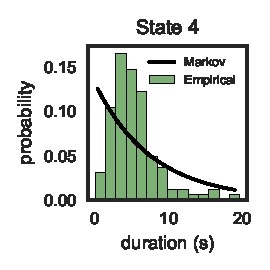
\includegraphics[width=1.8in]{figures/arhmm/durations_3.pdf}
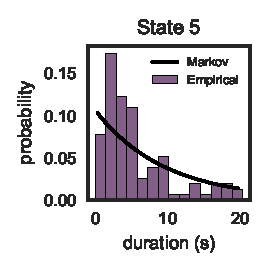
\includegraphics[width=1.8in]{figures/arhmm/durations_4.pdf}
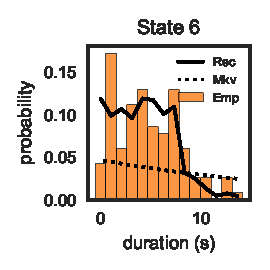
\includegraphics[width=1.8in]{figures/arhmm/durations_5.pdf}
\\
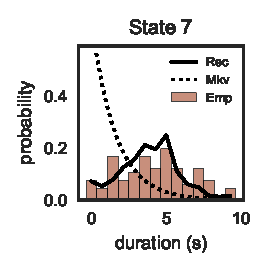
\includegraphics[width=1.8in]{figures/arhmm/durations_6.pdf}
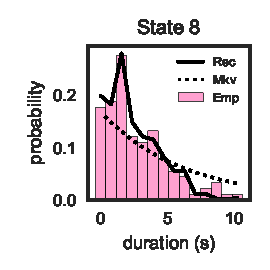
\includegraphics[width=1.8in]{figures/arhmm/durations_7.pdf}
\caption{Empirical distribution of state durations (histogram)
  compared to the geometric distribution implied by the Markovian
  weights of the transition model.  Some state durations are
  well-approximated by the geometric distribution, but others
  are peaked away from zero (e.g. states 2, 4, 6, and 7).  The
  recurrent transition model allows the AR-HMM to capture this
  non-Markovianity by modeling transitions as a function of location
  in latent state space~$x_t$. Solid lines show the distribution
  of simulated durations under the recurrent AR-HMM; dashed lines
  show the geometric duration distribution under the Markovian model.}
\label{fig:durations}
\end{figure}

Figure~\ref{fig:durations} shows histograms of the
empirical distribution of inferred state durations for each state. For
comparison, the solid lines show the distribution of
\emph{simulated} state distributions from our recurrent AR-HMM.  We
see a close correspondence. 

This correspondence is a direct result of the recurrent nature of the
model.  Without the recurrent terms, the state duration distributions
would necessarily follow the geometric distribution shown in dotted
black lines.  These distributions decay monotonically and cannot
capture the peaks away from zero that we find in the data.  This is
due to the fact that the distribution over durations~$d_k$ of
state~$k$ under a Markov model (ignoring the recurrent weights) is
given by,
\begin{align*}
  p_{k \to k} &= [\mathrm{softmax}(r_{k})]_k, \\
  d_k &\sim \mathrm{Geom}(1-p_{k \to k}).
\end{align*}
While some states (e.g. states 1, 5, and 8) seem to follow the Markov
assumption quite well, others (states 2, 4, and especially 7), are far
from Markovian.  The recurrent model incorporates the continuous
latent state~$x_t$ into the transition probabilities via the additive
term~$R x_t$ in the softmax and thereby captures the non-Markovianity.

\clearpage


\subsection{Inferred states overlap with those of~\citet{kato2015global}}


\begin{figure}[h]
\centering%
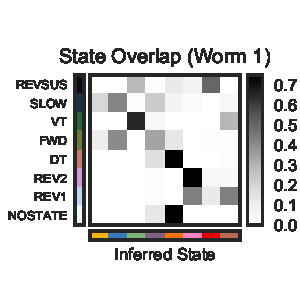
\includegraphics[width=1.9in]{figures/arhmm/overlap_0.pdf}
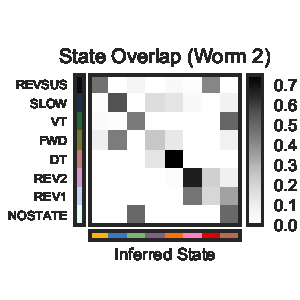
\includegraphics[width=1.9in]{figures/arhmm/overlap_1.pdf}
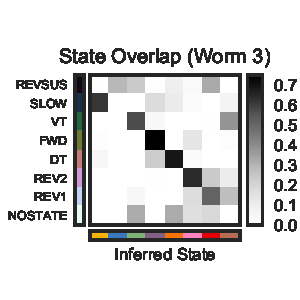
\includegraphics[width=1.9in]{figures/arhmm/overlap_2.pdf}
\\
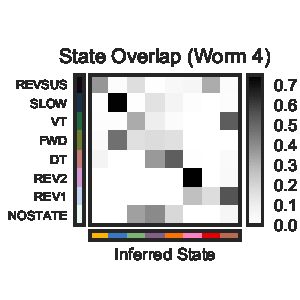
\includegraphics[width=1.9in]{figures/arhmm/overlap_3.pdf}
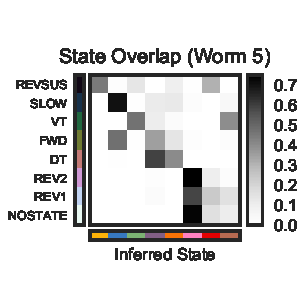
\includegraphics[width=1.9in]{figures/arhmm/overlap_4.pdf} 
\caption{Overlap between the manually labeled states of~\citet{kato2015global}
  and the inferred states of the AR-HMM. Each row is a normalized probability
  distribution over which of the~$K$ discrete states each worm was inferred to
  be in for the corresponding manual label.}
\label{fig:overlap}
\end{figure}

Figure~\ref{fig:overlap} shows a close correspondence between manually
labeled states and inferred discrete states, indicating that the
switching linear dynamics assumption is a formal specification of the
different dynamical modes reported by~\citet{kato2015global}.
Specifically, different ``behaviors'' correspond to different linear
dynamical regimes in continuous latent space.

A few patterns emerge here:
\begin{itemize}
\item Worm 3 differs from the rest, and seems to have a separate
  matching of inferred states and true states.  This list focuses
  on patterns in Worms 1, 2, 4, and 5. 
\item \textsf{REVSUS} --- the most common manually labeled state ---
  tends to overlap with the red and yellow inferred states.
\item \textsf{SLOW} --- the second most common --- and \textsf{FWD}
  often map onto the blue state.
\item \textsf{VT} (ventral turns) map to the green state, which
  has a rise and fall of activity in cluster 3 (neurons
  {\sf ALA, ASKL, ASKR, RIVL, RIVR, SMDVL} and \textsf{SMDVR}).
  This seems consistent with the roles of sensory neurons~\textsf{ASK*},
  interneurons \textsf{RIV*}, and motor neurons \textsf{SMDV*} in
  local search behavior.
\item Skipping ahead, \textsf{DT} (dorsal turns) often map onto
  the orange and, to a much lesser extent, the purple state. Both
  states encourage upswings in cluster 4 ({\sf SMBDL, SMBDR, SMBVL, SMBVR}, and \textsf{URYVR}).
  The first four of these neurons are motor neurons involved in
  local search behavior. 
\item In addition to the blue state, \textsf{FWD} maps onto the
  green, purple, and orange states as well, though much less significantly.
\item \textsf{REV2} and \textsf{REV1} map primarily onto the pink state.
  This state is characterized by an excursion of activity along cluster
  1 ({\sf AVAL, AVAR, BAGL, RIML, RIMR, SAAVR, SABVL, SABVR, VA01}.
  The \textsf{AVA*} interneurons innervate motor neurons.
  \textsf{RIM*} are motor neurons that modulate reversals.
  \textsf{SABV*} are interneurons and sublateral motor neurons.
  \textsf{VA01} is a motor neuron.

  We also note that \textsf{REV1} maps onto the brown state, which
  is also associated with ventral turns. Judging by the dynamics plots above,
  it seems ventral turns are often followed by type-1 reversals.
\item \textsf{NOSTATE} seems to often map in different ways across worms.
  This is by far the least common of the manually-labeled states.
\end{itemize}

\todo[inline, size=\normalsize]{Combining these overlap figures
  with the transition matrices above, I find a slightly different
  transition structure from what was reported in Kato et al Figure 4E.
  I find that the transitions between \textsf{REVSUS} and \textsf{FWD}
  are largely mediated by the \textsf{SLOW} state without an intervening
  turn.  I find that ventral turns are often exercised in between
  \textsf{REVSUS} and \textsf{REV1}, and that dorsal turns are often
  used between episodes of forward crawling.  Does this make any sense?
  }

\clearpage

% \subsection{Inferred change-points also match manual labels}

% \begin{figure}[h]
% \centering%
% 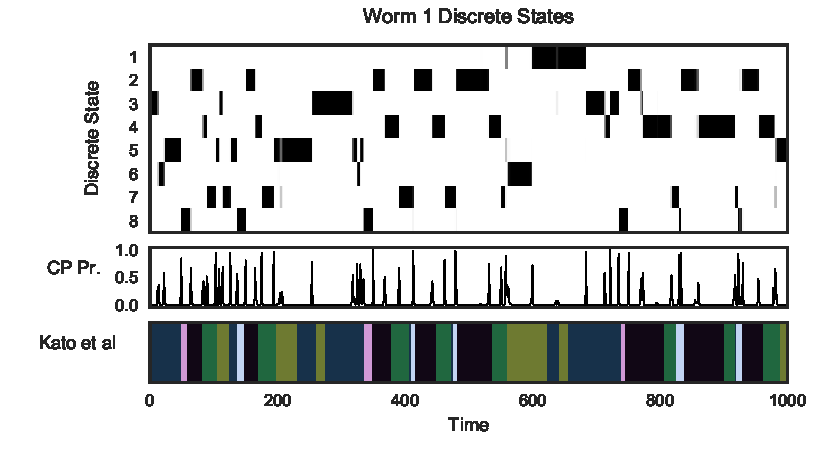
\includegraphics[width=5.5in]{figures/arhmm/z_cps_worm0.pdf}
% 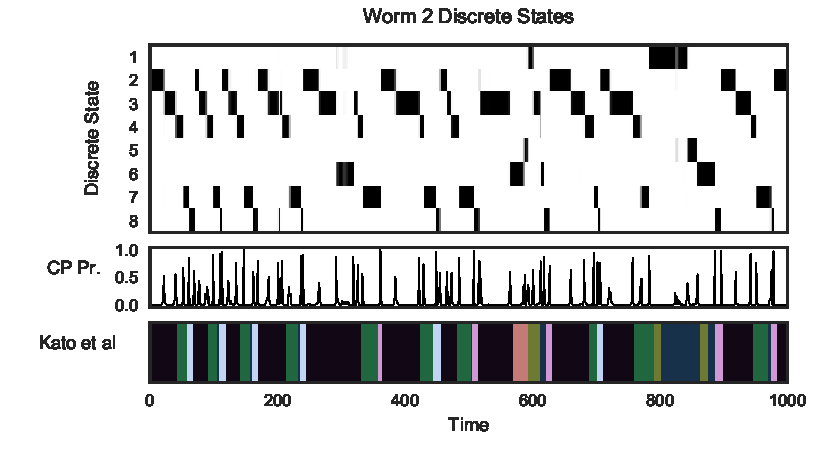
\includegraphics[width=5.5in]{figures/arhmm/z_cps_worm1.pdf}
% \caption{(top) Posterior distribution over latent states~$z_t$.
%   Each column corresponds to a time bin and sums to one.
%   (middle) The posterior probability of change-points.
%   (bottom) For reference,
%   the manually labeled states of~\citet{kato2015global}. Colors match those
%   of Figure~\ref{fig:overlap}.}
% \label{fig:z_cps_12}
% \end{figure}

% Figures~\ref{fig:z_cps_12}, \ref{fig:z_cps_34}, and \ref{fig:z_cps_5}
% show the posterior distribution of latent states~$z$ inferred from
% neural activity alone. From this posterior, we also compute the probability
% of a change-point, where~$z_{t+1} \neq z_t$.  For reference, we show the
% manually labeled states of~\citet{kato2015global} below. Here, patterns
% like the cascade from states 2 to 3 to 4 (red to yellow to green) are
% apparent. 

% \begin{figure}[h]
% \centering%
% \includegraphics[width=5.5in]{figures/arhmm/z_cps_worm2.pdf}
% \includegraphics[width=5.5in]{figures/arhmm/z_cps_worm3.pdf}
% \caption{See Figure~\ref{fig:z_cps_12} caption.}
% \label{fig:z_cps_34}
% \end{figure}

% \begin{figure}[h]
% \centering
% \includegraphics[width=5.5in]{figures/arhmm/z_cps_worm4.pdf}
% \caption{See Figure~\ref{fig:z_cps_12} caption.}
% \label{fig:z_cps_5}
% \end{figure}

% \clearpage

\subsection{Inferred states change-points correspond with changes in dynamics}

Figures~\ref{fig:segmentation_1} through~\ref{fig:segmentation_5} show an
interval of latent state trajectories~$x$ along with the segmentation from
the inferred discrete states~$z$ (top).  For comparison, we also show the
manual segmentation of~\citep{kato2015global} (bottom).  The inferred
segmentation seems to identify change-points when one or more of the latent
continuous states changes dynamics.  Indeed, this is the assumption of the
model.  By contrast, the segmentation of~\citep{kato2015global} is based on
a read-out of a single neuron, and while it is largely consistent with the
inferred segmentation at the population level, it misses some salient
changes in dynamics.  For example, see the inferred change-point around
time 700 in worm 1.  This change-point was not identified in the manual
data.

\begin{figure}[h]
\centering%
\includegraphics[width=5.5in]{figures/arhmm/x_segmentation_0.pdf}
\includegraphics[width=5.5in]{figures/arhmm/x_segmentation_zimmer_0.pdf}
\caption{Latent state trajectories superimposed on the inferred segmentation (top)
  and the manual segmentation (bottom).}
\label{fig:segmentation_1}
\end{figure}


\begin{figure}[h]
\centering%
\includegraphics[width=5.5in]{figures/arhmm/x_segmentation_1.pdf}
\includegraphics[width=5.5in]{figures/arhmm/x_segmentation_zimmer_1.pdf}
\caption{See caption of Figure~\ref{fig:segmentation_1}}
\label{fig:segmentation_2}
\end{figure}


\begin{figure}[h]
\centering%
\includegraphics[width=5.5in]{figures/arhmm/x_segmentation_2.pdf}
\includegraphics[width=5.5in]{figures/arhmm/x_segmentation_zimmer_2.pdf}
\caption{See caption of Figure~\ref{fig:segmentation_1}}
\label{fig:segmentation_3}
\end{figure}


\begin{figure}[h]
\centering%
\includegraphics[width=5.5in]{figures/arhmm/x_segmentation_3.pdf}
\includegraphics[width=5.5in]{figures/arhmm/x_segmentation_zimmer_3.pdf}
\caption{See caption of Figure~\ref{fig:segmentation_1}}
\label{fig:segmentation_4}
\end{figure}


\begin{figure}[h]
\centering%
\includegraphics[width=5.5in]{figures/arhmm/x_segmentation_4.pdf}
\includegraphics[width=5.5in]{figures/arhmm/x_segmentation_zimmer_4.pdf}
\caption{See caption of Figure~\ref{fig:segmentation_1}}
\label{fig:segmentation_5}
\end{figure}
\clearpage



\clearpage
\bibliography{refs}
\bibliographystyle{abbrvnat}

\end{document}
